\subsection{Fase 2: Metaheurística de optimización multiobjetivo} \label{sec:3:metaheurística}
Se trata del núcleo principal del presente proyecto, pues trata de dar solución al problema en sí mediante un enfoque de metaheurísticas.

Como ya se ha introducido previamente, estamos ante un problema de \textit{timetabling/scheduling} que son generalmente problemas complejos debido a su naturaleza combinatoria.
Matemáticamente se dice que pertenecen al conjunto de los problemas llamados \textit{NP-Duros (NP-Hard)}, pues los algoritmos clásicos empleados para resolverlos tienen una complejidad al menos de tipo exponencial.

Clásicamente se han empleado algoritmos para problemas concretos de este tipo que van desde el \textit{General Scheduling Problem} (GSP) que es el caso más general hasta los casos más concretos mediante variaciones respecto al anterior, haciéndolo más o menos restrictivo.
Algunos son: el \textit{Open Shop Scheduling} (OSS), \textit{Job Shop Scheduling} (JSS), \textit{Flow Shop Scheduling} (FSS) o \textit{Permutational Flow Shop Scheduling} (PFSS). Una clasificación más detallada de este tipo de problemas clásicos se encuentra en~\cite{sota:tesis-doctoral}.

Lejos del entorno académico, los problemas reales de \textit{scheduling} (como el que tenemos entre manos en este TFM) pueden ser muy diferentes entre sí, habiendo pues mucha variedad en función del ámbito de aplicación.
Por ejemplo, se han estudiado casos para transporte público~\cite{sota:transporte-publico} o universidades~\cite{sota:universidad} y podemos ver cómo son completamente diferentes en cuanto a restricciones y necesidades de cada una de las soluciones, por lo que las metodologías empleadas para su resolución son bien diferentes.

Existen gran cantidad de técnicas que se han empleado previamente para resolver este tipo de problemas, comenzando por sencillos heurísticos aplicados a los problemas clásicos bien estudiados y formalizados, pero este tipo de algoritmos solamente son aplicables a instancias pequeñas debido a la mencionada naturaleza no polinómica, por lo que no son útiles en problemas reales. Por otro lado, se ha analizado cómo transformar un problema de \textit{scheduling} en un problema de coloreado de grafos~\cite{sota:estudio-coloreado-grafos, sota:algotimo-coloreado-grafos}, lo que nos permite emplear los algoritmos existentes para este tipo de problemas, entre los que podemos encontrar exactos y aproximados.

También existen enfoques más modernos que emplean técnicas de \textit{Aprendizaje Automático} habitualmente combinados con metaheurísticas~\cite{sota:machine-learning-geneticos} y recientemente \textit{Hiperheurísticas} (como por ejemplo en~\cite{sota:hiperheuristicas}). En el libro~\cite{sota:libro-sota-scheduling} se encuentran explicadas de forma detallada todas estas técnicas aquí nombradas.

Por último, la técnica más empleada actualmente para resolver este tipo de problemas son las metaheurísticas: una familia de algoritmos de carácter genérico empleados como \textit{framework} para resolver un problema dado enfocándolo como un problema de optimización. Tienen dos características principales~\cite{sota:metaheuristicas}:

\begin{enumerate}
    \item En contraposición a los heurísticos, no dependen directamente del problema específico, únicamente han de ser adaptados parcialmente.
    \item Por definición son métodos de búsqueda aproximados, que tratan de combinar técnicas de exploración y explotación (véase la \autoref{capitulo:3:busqueda-divers-intens}) para obtener la mejor solución posible dentro del espacio de búsqueda definido.
\end{enumerate}

Tienen dos conceptos básicos que conforman la clave para su implementación para un problema concreto: la codificación y la función objetivo.

La codificación permite representar una solución de la forma más compacta posible sin perder información del dominio. Una buena codificación tendrá las siguientes características~\cite{sota:metaheuristicas-design-impl}:

\begin{itemize}
    \item \textit{Completitud}: Todas las soluciones asociadas con el problema deben poder ser representadas. Se debe garantizar una representatividad total dentro del espacio de soluciones. Si no es definida correctamente podría haber soluciones incapaces de ser representadas y lógicamente afectará a la eficiencia de la metaheurística.
    \item \textit{Conectividad}: Debe existir un método que permita moverse entre dos soluciones del espacio de búsqueda, de forma que cualquier solución del espacio pueda ser alcanzada (en especial el óptimo global).
    \item \textit{Eficiencia}: Fácil de manipular por los operadores de la búsqueda (definidos por cada metaheurística).
\end{itemize}

Por otro lado, las metaheurísticas emplean una o varias soluciones que son comparadas entre sí empleando una función objetivo o de evaluación (en inglés denominada \textit{fitness}), que representa el objetivo de la búsqueda, de forma que si nos enfrentamos a un problema con varios parámetros objetivo, podamos ponderarlos u ordenarlos según los criterios que se adecúen al problema. Existen varios enfoques para definir una función de evaluación de un problema multiobjetivo: enfoques escalares, basados en criterios, basados en dominaciones (óptimos de Pareto) entre las soluciones o basados en indicadores de calidad. Los más sencillos son los primeros, pues permiten trasformar el problema multiobjetivo en uniobjetivo y al ser el empleado en este TFM será descrito con mayor detenimiento en el \autoref{apartado:adaptacion-fitness}

Un problema de optimización multiobjetivo es de la siguiente forma:
%\[
\begin{flalign*}
    & \max_{x} \quad \textbf{f(x)} = \left( \, f_1(\textbf{x}), f_2(\textbf{x}), f_3(\textbf{x}), \dots, f_n(\textbf{x}) \, \right) \,,\\
    & \; \text{s.a.} \quad \textbf{x} \in X
\end{flalign*}
%\]
siendo $X$ el conjunto de soluciones factibles, definido mediante una serie de restricciones dadas por el dominio del problema.

La función de evaluación es dependiente del problema a resolver y suele ser de un coste computacional importante.

Estas técnicas fueron muy innovadoras, pues permitieron la resolución de muchos problemas clásicos que hasta entonces no podían resolverse con técnicas clásicas. Además, soportan perfectamente instancias grandes, por lo que hasta la fecha es la técnica más prometedora para el problema a resolver en este TFM.

No obstante, la mayor desventaja de las metaheurísticas es que, al tratarse de métodos aproximados, no garantizan que se encuentre una solución óptima global ni que se encuentre acotada en algún rango de valores~\cite{sota:metaheuristicas-design-impl} como sí permiten otras técnicas. 
%Un inconveniente frente a todas las posibilidades que las metaheurísticas nos ofrecen. % RELIMINADO REV 0.3.2

Una vez decidida la técnica a emplear para resolver el problema definido, el siguiente paso es elegir de entre el catálogo de metaheurísticas existentes hasta la fecha, una de ellas. A lo largo del tiempo se han ido proponiendo diferentes taxonomías para ordenar toda esta gran cantidad de metaheurísticas.
Así, una de las clasificaciones más conocidas es la propuesta por Osman en~\cite{metaheuristicas:taxonomia1} que distingue entre aquellas basadas en búsquedas locales (pequeños cambios a una misma solución), las constructivas (en cada iteración se van añadiendo partes que al final conforman una solución al completo) y las poblacionales (se combinan varias soluciones entre sí).

Gendreau y Potvin~\cite{metaheuristicas:taxonomia2} propusieron en 2005 una clasificación dicotómica: aquellas de tipo trayectorial y de tipo poblacional, combinando así las de búsqueda local y las constructivas en un mismo grupo que emplea únicamente una sola solución por iteración mientras que las segundas emplean un conjunto dinámico de soluciones que en cada iteración irá cambiando.

Existen otras clasificaciones menos relevantes que dividen las metaheurísticas en aquellas inspiradas en la naturaleza y las que no, si emplean capacidad de memoria o no, o si son de naturaleza determinista o estocástica. Una de las últimas clasificaciones~\cite{sota:metaheuristicas} propone la división en metafóricas (metáforas de la biología, química, música, matemáticas, física o social-deportiva) o no metafóricas.

En el caso de este TFM, la elección fue de carácter histórica: los proyectos previos habían empleado dos metaheurísticas \textit{Recocido Simulado (\sa{}, SA)} y del \vns{} (\textit{Búsqueda de Entornos Variable}), en los que esta última obtenía resultados más prometedores que la otra.

El SA es una metaheurística trayectorial de búsqueda local basada en la aceptación de soluciones peores con una cierta probabilidad que depende del valor de un parámetro llamado \textit{temperatura} que varía con el tiempo (cada cierto número de iteraciones) una cantidad constante (o variable en algunos casos) de forma que al final de la ejecución ya no se aceptan soluciones peores en ningún caso (probabilidad igual a cero), de esta forma en las primeras iteraciones la búsqueda será más diversificada y cuanto más tiempo transcurra irá disminuyendo y aumentando de manera complementaria la intensificación. Al igual que el VNS, parte de una solución inicial dada, ya sea generada aleatoriamente o mediante una heurística más sofisticada; pero a diferencia de este, se mueve hacia otras empleando un único entorno. Esta es la mayor limitación de esta metaheurística y por ello hemos planteado la alternativa del uso de un VNS, partiendo así de la hipótesis~\ref{H2}, que sugiere que empleando más entornos se mejoran los resultados del SA\@.% "\@" porque acaba en mayúscula la frase

\subsubsection{Búsqueda en Entornos Variables (VNS)} \label{sec:vns}
Se trata de una metaheurística trayectorial, pues maneja una única solución en cada iteración, además de tipo búsqueda local pues trata de modificarla iterativamente para mejorarla empleando un catálogo de \textit{entornos} o vecindades (\textit{neighborhoods}). A su vez es de tipo no metafórica: no se inspira en ningún proceso de la naturaleza. Es además de tipo estocástico y no emplea memoria para su funcionamiento.

Su nombre radica precisamente en sus dos conceptos fundamentales: búsqueda local y entornos variables. En su versión original~\cite{vns} se fundamenta en dos etapas: \textit{descenso} y \textit{perturbación}, la primera consiste en el intercambio sistemático del entorno empleado durante una búsqueda local simple que nos permite alcanzar un óptimo local; mientras que la segunda radica en la alteración aleatoria de la solución para evitar atascarse en óptimos locales evitando así una convergencia prematura. Ambas serán descritas en detalle más adelante en esta sección.

Así pues, el VNS parte de una lista predefinida de entornos, que definen el criterio a emplear para moverse entre soluciones a partir de una inicial. Al entorno $k$ del conjunto de vecindades se les suele denotar como $N_k, \; k=1,\dots,k_{max}$ y al conjunto de soluciones alcanzables mediante la vecindad $k$ como $N_k(x)$.
Un ejemplo sencillo de entorno podría ser en el caso de una optimización de una variable en el dominio $\mathbb{R}$: dos posibles entornos serían $N_1=[x-2, x+2]$ y $N_2=[x-7, x+7]$, ilustrados en la \autoref{fig:ejemplos-entorno}.

\begin{figure}[htbp]
    \centering
    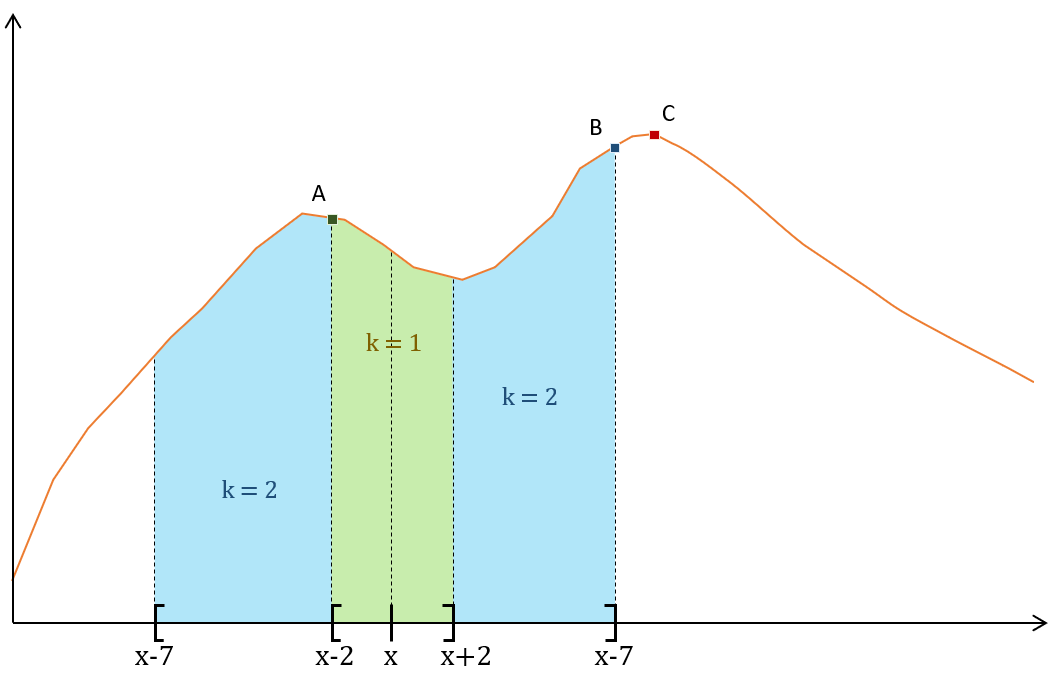
\includegraphics[width=\linewidth]{ejemplos-entorno}
    \caption{Ejemplo de dos entornos definidos en $\mathbb{R}$}
    \label{fig:ejemplos-entorno}
\end{figure}

Como podemos observar, los entornos se definen con respecto a una solución, denotada por $x$. En el ejemplo, los entornos se han definido de forma que el conjunto de soluciones alcanzables mediante el segundo sea un superconjunto de aquel empleando el primero, ampliando de esta forma las fronteras de la búsqueda (no es necesario definirlos así, pero suele ser una práctica habitual). Si lanzamos una búsqueda local sobre la función del ejemplo empleando el entorno $k_1$, el punto más óptimo que podemos alcanzar en caso de maximización es el punto $A$, mientras que si empleamos el $k_2$ será el $B$. El punto $C$ es el óptimo global de la función, que no es alcanzado por ninguno de los entornos definidos, aunque $k_2$ se aproxima bastante.

Con todo, el VNS se basa en tres características \cite{vns}:

\begin{enumerate}
    \item Un óptimo local respecto a una estructura de vecindad no necesariamente lo es respecto a otra.
    \item Un óptimo global es a su vez óptimo local respecto a todas las posibles estructuras de entornos.
    \item Empíricamente se ha determinado que para la mayoría de problemas, los óptimos locales con la misma o distinta estructura de entornos están relativamente cerca.
\end{enumerate}

En la \autoref{fig:VNS-facts} se ilustran estas tres características visualmente.

\begin{figure}
    \centering
    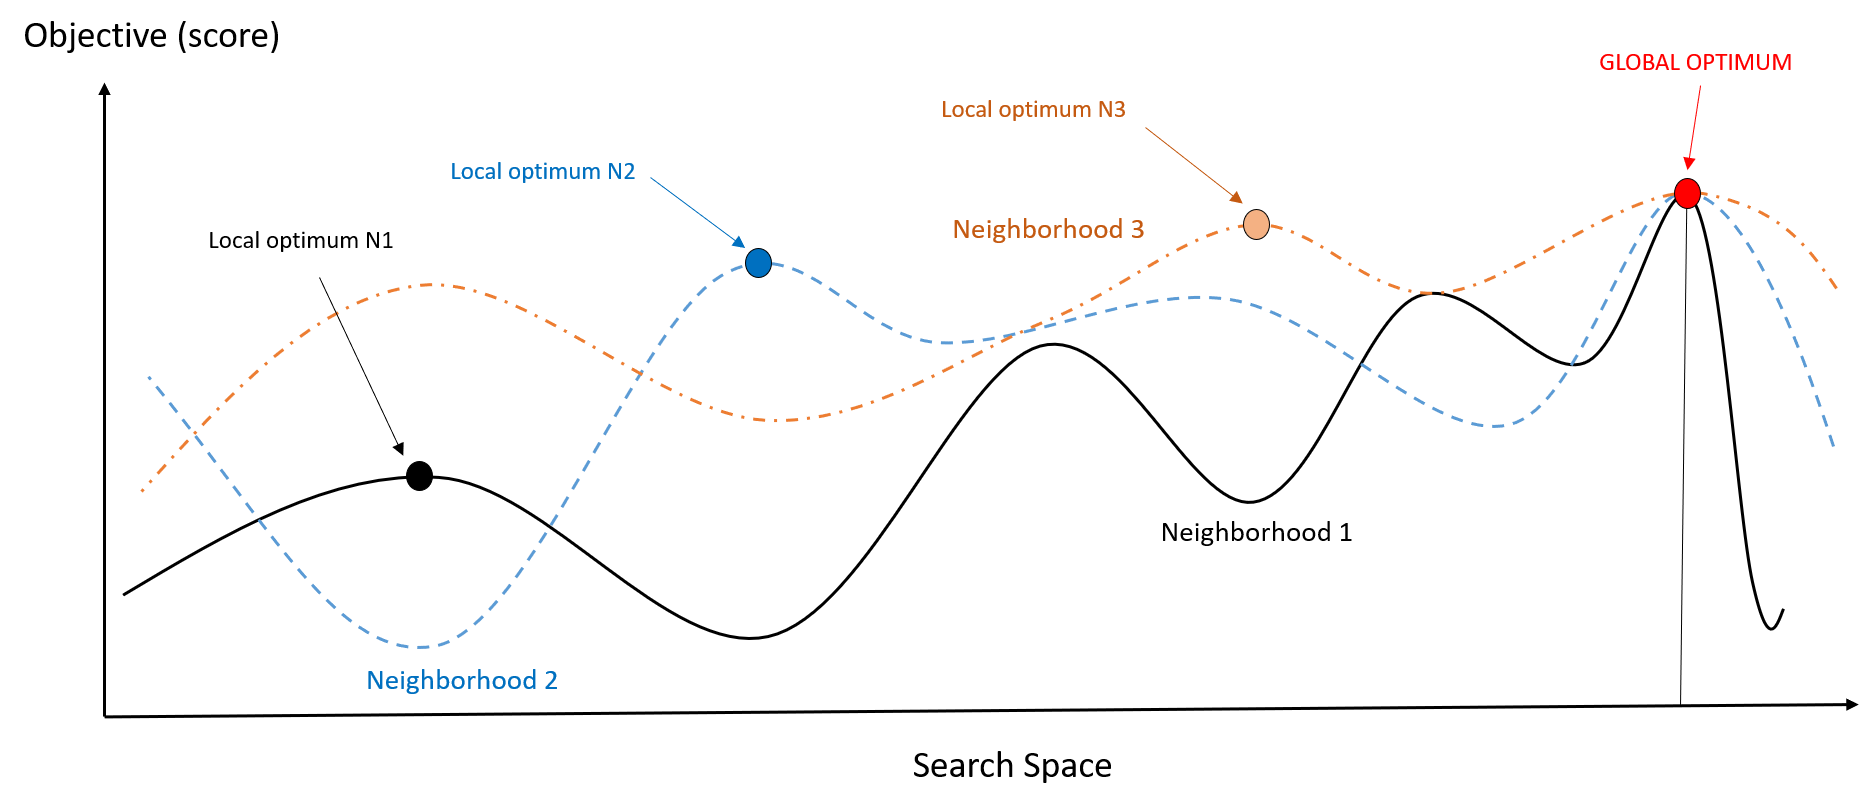
\includegraphics[width=\linewidth]{VNS-facts}
    \caption[Ilustración que representa las características sobre las que se fundamenta el VNS]{Ilustración que representa las características sobre las que se fundamenta el VNS.}
    \label{fig:VNS-facts}
\end{figure}

Comenzaremos analizando el cambio entre entornos, que se lleva a cabo de la misma forma en todo VNS siguiendo el \autoref{algoritmo:VNS-cambio-entornos}. La \autoref{fig:esquema-idea-basica-VNS} muestra lo mismo de forma más gráfica.
Como se puede observar, se llevan a cabo acciones diferentes en función de si la nueva solución obtenida por el algoritmo de búsqueda local es mejor o peor que la de partida: si la nueva solución generada mediante la vecindad actual es mejor, se reinicia; mientras que si es peor o igual, se amplía la búsqueda al siguiente entorno. La función fitness se ha denotado como $f(x) \in [0,1]$.

\begin{figure}
    \centering
    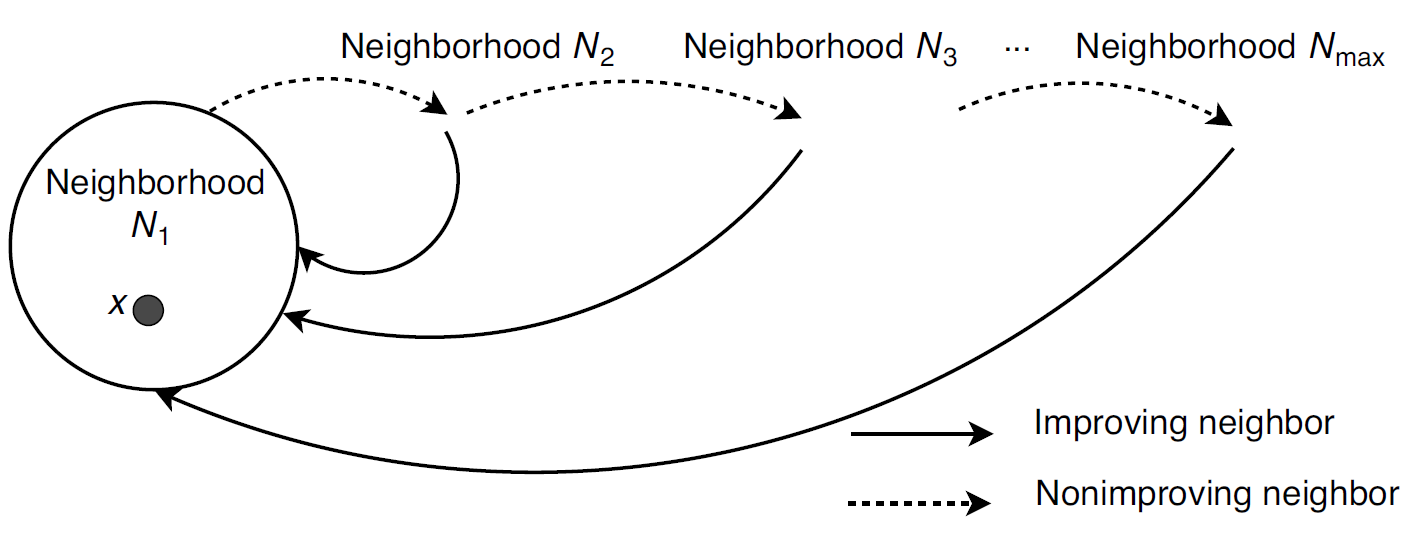
\includegraphics[width=.9\linewidth]{esquema-idea-basica-VNS}
    \caption[Esquema que representa la idea básica del cambio de entornos en todo VNS]{Esquema que representa la idea básica del cambio de entornos en todo VNS. Fuente:~\cite{sota:metaheuristicas-design-impl}}
    \label{fig:esquema-idea-basica-VNS}
\end{figure}

\begin{algorithm}[htbp]
    \caption{Algoritmo del cambio de vecindades empleado por el VNS en el caso de un problema de maximización}
    \label{algoritmo:VNS-cambio-entornos}

    \DontPrintSemicolon
    \KwData{

    $x$, solución actual. En la primera iteración es la inicial.

    $x'$, solución obtenida del algoritmo de búsqueda local con el entorno $k$

    $k$, índice de la vecindad actual
    }
    \medskip

    \SetKwFunction{FNeighbourhoodChange}{NeighbourhoodChange}
	\SetKwProg{Fn}{Función}{:}{}
	\Fn{\FNeighbourhoodChange{$x$,$x''$,$k$}}{	
	  \If{$f(x')>f(x)$}{
			$x \leftarrow x'$  \Comment{Moverse a la mejor solución}
			$k \leftarrow 1$  \Comment{Reinicio de vecindades}
		}
		\Else{
			$k \leftarrow k+1$  \Comment{Siguiente vecino}
		}	
	}


\end{algorithm}

No necesariamente un entorno amplio, es decir, con mayor conjunto de soluciones factibles, es mejor que uno más reducido, pues el espacio de búsqueda es mayor y esto repercutirá decisivamente en el rendimiento del algoritmo de búsqueda. Además, en problemas reales, con un mayor número de variables, el espacio de búsqueda es mucho más complejo y difícil de explorar. Es por ello que lo más conveniente es emplear las vecindades más sencillas y pequeñas al principio de forma que solo se pasa a las más grandes y costosas en caso de que las anteriores no resulten fructíferas.

En función de los subprocesos que se utilicen durante la búsqueda estaremos hablando de un tipo de VNS u otro. A continuación, describiremos las características de aquellos tipos de VNS que se han implementado en este TFM\@.

El VNS en su versión básica (conocido como \textit{Basic VNS}) se compone de dos fases: la búsqueda local y la ``agitación'' (\textit{shake}) siendo la primera determinista y la segunda estocástica. Una componente aleatoria aporta nueva información a la búsqueda que podría ser de ayuda a la componente determinista.

La componente de búsqueda local se puede realizar en dos enfoques diferentes: buscando la primera solución que mejore la actual (\textit{First Improvement}) o empleando la mejor de todas las posibles soluciones del entorno (\textit{Best Improvement}). Sin embargo no siempre es posible obtener todas las soluciones posibles de un entorno, especialmente en problemas complejos como el que tenemos entre manos. 

En este problema se ha empleado una técnica mixta que si bien no emplea la mejor solución, tampoco emplea la primera mejor, sino que continúa la búsqueda hasta que la solución no se mejore en un porcentaje de tolerancia (véase la \autoref{apartado:condiciones-parada} para una descripción detallada).

Los Algoritmos~\ref{algoritmo:BestImprovement} y~\ref{algoritmo:FirstImprovement} se han obtenido directamente de Hansel et al.~\cite{vns} y describen el proceso asociado al \textit{Best Improvement} y al \textit{First Improvement} respectivamente.

\begin{algorithm}[htbp]
    \caption{Best Improvement (maximización)}
    \label{algoritmo:BestImprovement}

    \DontPrintSemicolon
    \KwData{
    $x$, solución actual.
    }
    \medskip

    \Repeat{
    $f(x) \le f(x')$
    }{
    $x' \leftarrow x$ \;
    $x \leftarrow \arg \max_{y \in N(x')} f(y)$ \;
    }
    \Return x \;

\end{algorithm}

\begin{algorithm}[htbp]
    \caption{First Improvement (maximización)}
    \label{algoritmo:FirstImprovement}

    \DontPrintSemicolon
    \KwData{
    $x$, solución actual.
    }
    \medskip

    \Repeat{
    $f(x) \le f(x')$
    }{
    $x' \leftarrow x$ \;
    $i \leftarrow 0$ \;
    \Repeat{$f(x) > f(x')$ ó $i = |N(x)|$}{
    $i \leftarrow i + 1$ \;
    $x \leftarrow \arg \max \left\lbrace f(x), f(x^i)\right\rbrace $, $x^i \in N(x)$ \;
    }
    }
    \Return x \;

\end{algorithm}

Por otro lado, la componente estocástica introduce en la búsqueda una solución generada de forma aleatoria, de manera que se introduce nueva información en el proceso de búsqueda que puede mejorar el valor de fitness empleando, por ejemplo, fragmentos de solución aleatorios que de forma determinista nunca podrían haberse logrado o como mínimo habría sido necesario un mayor tiempo de cómputo.

En el \autoref{algoritmo:Basic-VNS} se muestra el proceso esquemáticamente para el VNS Básico. Nótese que la condición de parada es únicamente el tiempo de cómputo, no obstante, se suele combinar con un porcentaje mínimo de mejora de forma que si la búsqueda se estanca, no se pierda tiempo de cómputo innecesariamente. Las condiciones de parada del algoritmo se encuentran descritas en profundidad en la \autoref{apartado:condiciones-parada}.

\begin{algorithm}[htbp]
	\caption[Basic VNS]{Basic VNS~\cite{vns}}
	\label{algoritmo:Basic-VNS}
	
	\DontPrintSemicolon
	\KwData{
		
		$x$, solución actual. 
		
		$k_{max}$, número de entornos definidos para la metaheurística.
		
		$t_{max}$, tiempo máximo de ejecución del algoritmo.
	}

%	\medskip
	\bigskip
	
	$t \leftarrow 0$ \;
	
	\While{$t<t_{max}$}{
		
		\Repeat{
			$k = k_{max}$
		}{
			$x' \leftarrow \texttt{Shake}(x,k)$ \Comment{Componente estocástica}
			$x'' \leftarrow \texttt{FirstImprovement}(x')$ \Comment{Búsqueda local}
			$x,k \leftarrow \texttt{NeighbourhoodChange}(x,x'',k)$ \Comment{Cambio de vecindad}
		}
		$t \leftarrow \texttt{CpuTime}()$ \Comment{Medición del tiempo de ejecución}
	}
	
	\Return x \;
	
\end{algorithm}

El VNS en su versión básica fue propuesto en 1997 por Hansen y Mladenovi\'{c} en~\cite{vns1997}. Sin embargo, dado que cada problema es diferente y se adapta mejor a un método u otro, con el tiempo los propios autores han definido algunas variaciones, propuestas en~\cite{vns1999, vns2003}, y que serán descritas a continuación.

La forma más sencilla de variar el método es suprimir una de las dos componentes: si eliminamos la componente estocástica, dejando la búsqueda únicamente determinista tenemos el \textit{Variable Neighborhood Descent} (VND); mientras que si la búsqueda es únicamente estocástica tenemos el \textit{Reduced Variable Neighborhood Search} (RVNS). Éste último es el menos costoso computacionalmente, sin embargo, es el que emplea menos información del problema, y su rendimiento suele ser peor que los demás.

Otra posible variación respecto a la versión básica se basa en emplear una técnica distinta para la búsqueda local. Si por ejemplo empleamos otro VNS únicamente determinista, es decir un VND (descent) en lugar de una búsqueda local simple, estaremos empleando un \textit{General VNS} (GVNS).



Por último, existen otras variaciones que rompen con la estructura básica del VNS, pero que se ha visto que dan buenos resultados para ciertos problemas, mejorando las variaciones anteriores. Entre ellas, el \textit{Skewed VNS} (SVNS) definido en~\cite{svns-def} cuya idea se basa en explorar óptimos locales lejanos a óptimo actual, potenciando la exploración sobre la explotación intrínseca al propio VNS por definición. Así, podrá moverse entre soluciones peores con el fin de encontrar información reutilizable en la solución. Sin embargo, la exploración no debe realizarse demasiado lejos de la solución actual, pues podría degenerar en una búsqueda de inicio múltiple (\textit{multistart}), donde se hacen búsquedas repetidamente empleando como solución de inicio una generada aleatoriamente, y esto se sabe que es ineficiente para este tipo de problemas~\cite{vns}). Para evitar esto, se define una función de distancia de forma que si la solución peor a explorar está demasiado lejos de la actual, se descarte.

Para ello, el SVNS define un parámetro adicional denotado normalmente como $\alpha$, que multiplica la función de distancia y que permite la exploración más o menos lejos de la solución actual. El \autoref{algoritmo:VNS-cambio-entornos} explicado previamente se redefine de la siguiente manera:

\begin{algorithm}[h]
    \caption{Redefinición del algoritmo de cambio de vecindades para un \textit{Skewed} VNS en un problema de maximización}
    \label{algoritmo:SVNS-cambio-entornos}

    \DontPrintSemicolon
    \KwData{

    $x$, solución actual. En la primera iteración es la inicial.

    $x'$, solución obtenida del algoritmo de búsqueda local con el entorno $k$

    $k$, índice de la vecindad actual

    $\alpha$, parámetro de la metaheurística
    }
    \bigskip

    \If{$f(x')+\alpha \cdot d(x,x') > f(x)$}{
    $x \leftarrow x'$ \Comment{Moverse a la mejor solución}
    $k \leftarrow 1$  \Comment{Reinicio de vecindades}
    }
    \Else{
    $k \leftarrow k+1$ \Comment{Siguiente vecindad}
    }

\end{algorithm}

Donde $\rho(x,x')$ es la función de distancia definida para el problema concreto.

El algoritmo central del SVNS es homólogo al \autoref{algoritmo:Basic-VNS} con la diferencia de que debido a que el nuevo algoritmo de cambio de entorno no retorna la mejor solución, sino la próxima a explorar (de peor \textit{fitness} pero alejada de ella), debemos almacenar la mejor para no perderla, y actualizarla en cada iteración. Además, será la que devolvamos al final del algoritmo.

Existen más variaciones del algoritmo básico del VNS que no se han contemplado en este proyecto, por lo que no se encuentran definidas aquí. Más información sobre estas puede hallarse en~\cite{vns}

\subsubsection{Adaptación del VNS al problema}
\label{apartado:adaptacion-VNS}

Recordemos que en secciones anteriores hemos definido la \faseuno{} que nos permite crear una solución inicial sobre la que el VNS pueda trabajar. El esquema planteado para la \fasedos{} se muestra en la \autoref{fig:esquema-fase2}, donde podemos ver cómo se combinan los algoritmos definidos previamente del VNS y el cambio de vecindad, junto a la condición de parada, definida \hyperref[apartado:condiciones-parada]{más adelante en esta sección}. El proceso denominado ``VNS concreto'' se trata del tipo de VNS elegido de entre todos los descritos previamente. Más adelante en el \autoref{capitulo:5} veremos cuál es el más eficiente de todos ellos.

\begin{figure}[htbp]
    \centering
    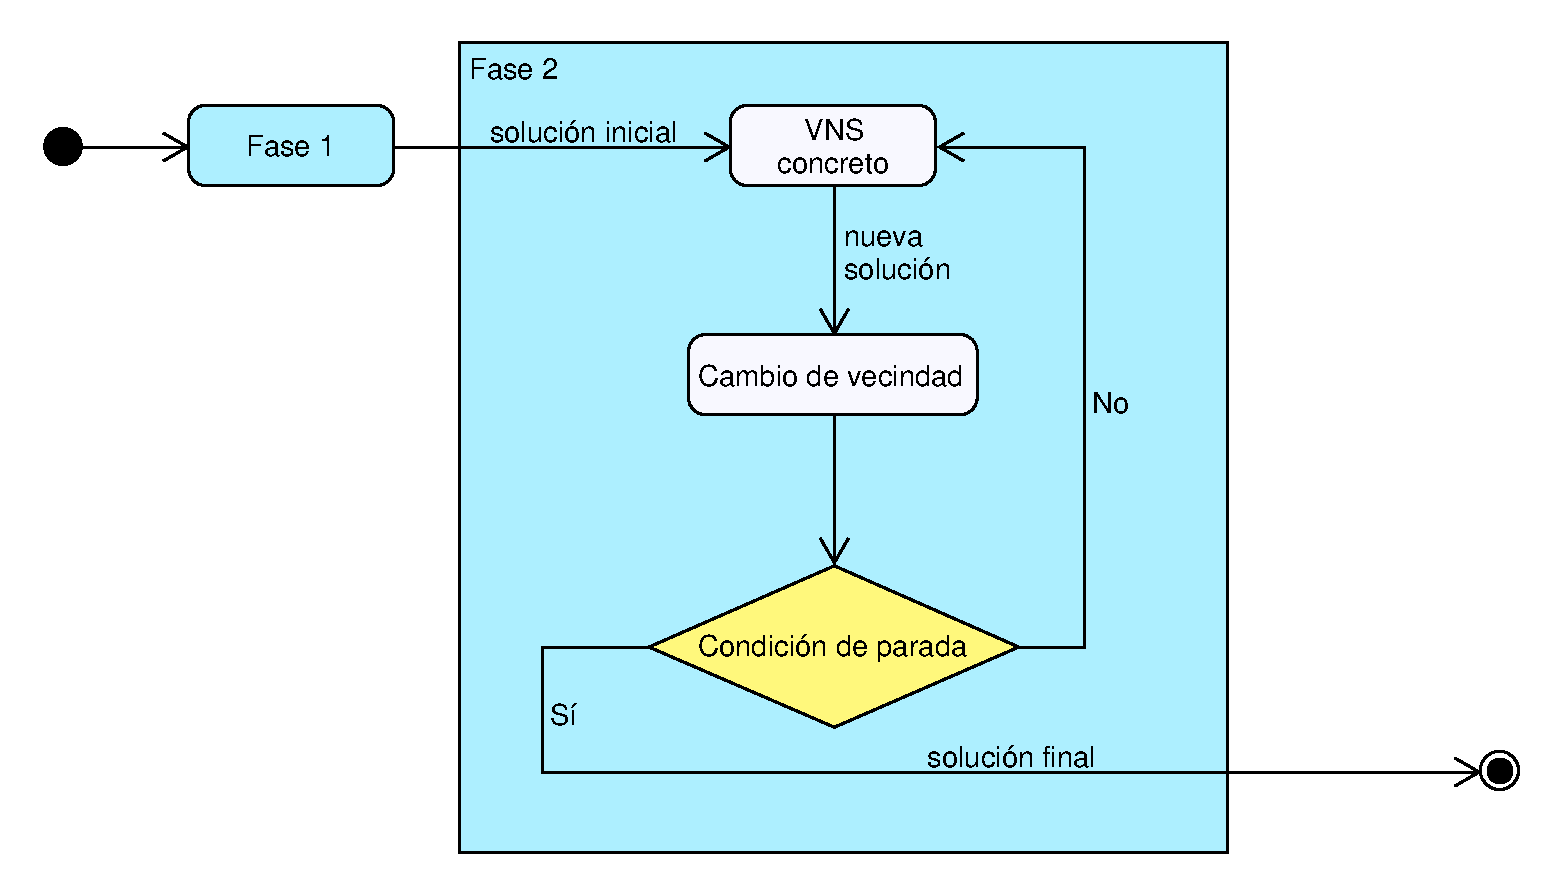
\includegraphics[width=\linewidth]{Esquema-Fase-2-centrico}
    \caption{Diagrama de flujo del funcionamiento de la Fase 2}
    \label{fig:esquema-fase2}
\end{figure}

\vspace*{\fill}

%Una vez definida la técnica a utilizar y las posibles variaciones planteadas, debemos instanciar los elementos del algoritmo y definir las heurísticas ---dependientes del problema concreto--- necesarias de la metaheurística.

En las próximas secciones se describe cómo se ha optado por adaptar la metaheurística descrita en la sección anterior al problema descrito en el \autoref{capitulo:2}: cómo se ha implementado la función de evaluación, qué entornos se han definido y bajo qué criterios son ordenados, las técnicas de exploración y explotación utilizadas, las condiciones de parada y la función de distancia para el caso del Skewed VNS.

La primera característica necesaria para las metaheurísticas ---y cualquier técnica, en palabras generales--- es la codificación (definida en la sección anterior). En el caso de nuestro problema, tal y como se describió detalladamente en la \autoref{sec:3:representacion-soluciones}, las soluciones se representan de forma matricial con una discretización del tiempo a intervalos de 5 minutos. La representación desde el punto de vista de la programación se encuentra descrita en la \autoref{sec:4:detalles-sistema}.

%Se han implementado todos los tipos de VNS descritos anteriormente, y empleando 3 tipos de entornos con subtipos variando ciertas restricciones. Los entornos se pueden seleccionar de dos formas diferentes, que más adelante compararemos su rendimiento: elección determinista (la clásica del VNS) y estocástica. Respecto a la búsqueda se impl

\paragraph{Función Fitness} \label{apartado:adaptacion-fitness}

La función fitness tiene por objeto la evaluación de una solución de manera que se puedan comparar entre sí dos o más soluciones del problema y poder decidir cuál es la mejor. Para poder definir una función de evaluación hacen falta uno o más \textit{objetivos} o \textit{criterios}. En caso de contar con un único objetivo, estaremos ante una búsqueda \textit{uniobjetivo}, mientras que si hay varios, sería \textit{multiobjetivo} o \textit{multicriterio}. En los problemas reales es habitual encontrarse con más de un criterio, normalmente contradictorios entre sí, por lo que aparece la figura del \textit{decisor}, que suele ser el cliente o el principal stakeholder del proyecto, y es el encargado de identificar aquellos objetivos que considere más relevantes (e incluso ponderarlos si es preciso), dando más peso dentro de la función a ciertos objetivos.

Otra opción para resolver esta situación consiste en presentar al decisor un conjunto de soluciones y que este elija la que más le convenga en función de sus preferencias. En nuestro caso, si bien podríamos haber optado por cualquiera de las dos decisiones, por razones históricas, se empleó la primera opción.

Dentro de la primera opción, tenemos diferentes alternativas introducidas \hyperref[sec:3:metaheurística]{al principio de esta sección}, que son: enfoques de escalarización, basados criterios, basados en dominaciones (óptimos de Pareto) entre las soluciones o basados en indicadores de calidad. Los más empleados son los primeros, pues aportan una mayor sencillez a la resolución del problema, ya que permiten trasformar el problema multiobjetivo en uniobjetivo. Dicha transformación se puede realizar a su vez de diferentes maneras, como se puede apreciar en la \autoref{fig:enfoques-fitness-multiobj}, definidas en detalle en~\cite{sota:metaheuristicas-design-impl} entre otros.

Nosotros hemos optado por el primero de todos, pues es el más sencillo y nos permite una mayor flexibilidad en caso de tener que modificar las prioridades de los objetivos en un futuro, sin necesidad de recalcular nada. El enfoque de escalarización mediante agregación construye la función fitness de la forma:

\begin{figure}
    \centering
    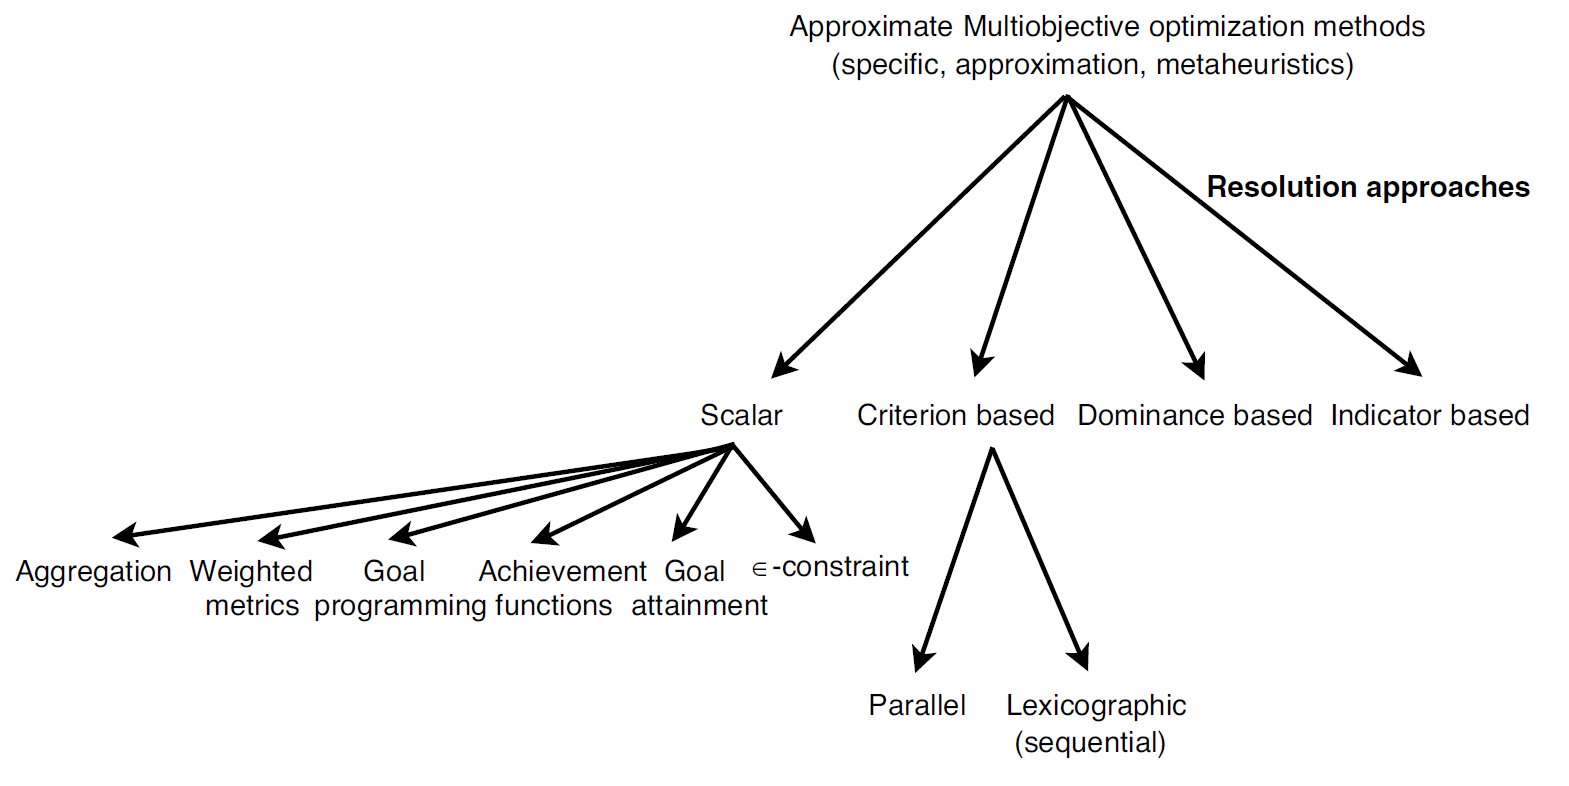
\includegraphics[width=\linewidth]{enfoques-resolucion-fitness-optimizacion-multiobj}
    \caption[Esquema de los posibles enfoques para la definición de la función fitness para casos de optimización multiobjetivo]{Esquema de los posibles enfoques para la definición de la función fitness para casos de optimización multiobjetivo. Obtenido de~\cite{sota:metaheuristicas-design-impl}}
    \label{fig:enfoques-fitness-multiobj}
\end{figure}
%
\[
    f(x) = \sum_{i=1}^{N} \lambda_i \cdot f_i(x) = \lambda_1 f_1(x) + \lambda_2 f_2(x) + \dots + \lambda_n f_n(x) + \dots
\]

donde $f_i(x)$ es la $i$-ésima función objetivo y $\lambda_i$ un escalar entre 0 y 1 de manera que~$\sum_{i=1}^n \lambda_i = 1$.

Cada función objetivo tiene asociado un escalar que pondera la relevancia de la misma, de manera que nuestro decisor, los responsables del proyecto por parte de \gls{CRIDA}, deberá ponderar los objetivos según sus criterios. En este caso, CRIDA aún no ha ponderado los objetivos, pero sí nos ha proporcionado una lista de los mismos ordenada por importancia, de forma que podemos utilizar diferentes valores para los pesos (escalares) siempre y cuando respetemos el orden de relevancia del decisor.

Los objetivos, ordenados del más prioritario al menos prioritario son:

\begin{enumerate}[label={O\arabic*}]
    \item \label{O1} Reducir el número de controladores. Si añadimos nuevos controladores imaginarios, debemos eliminarlos de forma que conservemos el número inicial y, si es posible, reducir el número inicial de los mismos.

    \item \label{O2} Factibilidad de las soluciones. Es importante que se cumplan las condiciones del dominio del problema, pero debido a que se trata de una planificación de urgencia, el decisor lo considera menos importante que el objetivo anterior.

    \item \label{O3} Tras el momento en el que se sucede la incidencia, los cambios propuestos por nuestro sistema deberían ser \textit{suaves}, es decir, que el número de cambios de sala de los controladores sea el menor posible.

    \item \label{O4} Cuanto más se parezca una solución del sistema a una plantilla mejor, pues los empleados están acostumbrados a manejar este tipo de planificaciones ya que resultan más intuitivas.
\end{enumerate}

%\begin{minipage}{\textwidth}
%
	Cuatro objetivos que podemos ponderar de diferentes formas. En este caso, en lugar de ponderarlos con valores aleatorios, se decidió tomar una técnica del estado del arte para la ponderación de objetivos en caso de que el decisor aporte información que permite su ordenación según importancia. Entre las posibles opciones encontramos:
    
    \begin{enumerate}[label=\alph*)]
        \item Mismos pesos para todos los objetivos, \textit{Equal Weights} (EW)~\cite{ew-paper}
        \item Pesos del método Rank-Sum (RS)~\cite{rs-rr-paper}
        \item Pesos del método Rank-Reciprocal (RR)~\cite{rs-rr-paper}
        \item Pesos del método \textit{Rank Order-Centroid} (ROC)~\cite{roc-paper}
    \end{enumerate}
%
%\end{minipage}

\NEW{El primero, \textit{Equal Weights}, se emplea en casos donde el decisor no aporte información de preferencia de objetivos. Los demás toman ese orden y nos permiten calcular el valor de cada peso mediante una fórmula diferente para cada uno.} 

\NEW{Una definición precisa y un estudio comparativo de estas técnicas de ponderación de objetivos, entre otras no nombradas, aplicables para problemas de decisión multiobjetivo, puede encontrarse en~\cite{ROC-comparativas-tecnicas,ROC-comparativas-tecnicas-upm}, donde podemos observar que una de las técnica que mejores resultados ofrece es el método ROC, por lo que será la que utilicemos.}

El método ROC utiliza la siguiente fórmula para la ponderación de cada objetivo $\lambda_i$ ordenados del más importante al menos importante:
\[
    \lambda_i = \sfrac{1}{N} \sum_{j=i}^N \frac{1}{j}
\]

%\begin{minipage}{\textwidth}
    Por lo tanto, calculamos todos los pesos $\lambda_i$ con $N=4$. Como podemos ver, suman $1$:
    \begin{flalign*}
        & \lambda_1 =  \sfrac{1}{4} \sum_{j=1}^4 \frac{1}{j} = \frac{1}{4} \left( \frac{1}{1}+\frac{1}{2}+\frac{1}{3}+\frac{1}{4} \right) = 0.52 \\
        &\lambda_2 =  \sfrac{1}{4} \sum_{j=2}^4 \frac{1}{j} = \frac{1}{4} \left( \frac{1}{2}+\frac{1}{3}+\frac{1}{4} \right) = 0.27 \\
        &\lambda_3 =  \sfrac{1}{4} \sum_{j=3}^4 \frac{1}{j} = \frac{1}{4} \left( \frac{1}{3}+\frac{1}{4} \right) = 0.15 \\
        &\lambda_4 =  \sfrac{1}{4} \sum_{j=4}^4 \frac{1}{j} = \frac{1}{4} \left( \frac{1}{4} \right) = 0.06
    \end{flalign*}
%\end{minipage}

Tres de las definiciones de las funciones objetivo han sido reutilizadas de diferentes partes del sistema \legacy{} (objetivos~\ref{O1},~\ref{O2} y~\ref{O4}). Esto es así debido a que, tal y como se detalló en la \autoref{capitulo:2:detalles-sistema}, el sistema \legacy{} también realizaba una optimización multiobjetivo que, debido a la ausencia de urgencia temporal de ejecución, el número de funciones objetivo era considerablemente mayor. 

En nuestro caso se han tomado aquellos objetivos decisivos para el sistema, aunando objetivos de diferentes fases de la metodología propuesta en el sistema \legacy{}. Véase~\cite{articulo1} para una mayor descripción tanto de la metodología \legacy{} como todas las funciones objetivo planteadas entonces, especialmente la normalización de las mismas, que se ha optado por no incluir aquí.

Adicionalmente, se ha creado un nuevo objetivo,~\ref{O3}, nacido de las nuevas características del presente sistema: el momento del cambio.


La función objetivo final, empleando el método de ponderación tiene esta forma:
\[
    \textbf{f}(\textbf{x})=
    %	\left\{
    \begin{cases}
        \lambda_1 f_1(\textbf{x}) + \lambda_2 f_2(\textbf{x}) + \lambda_3 f_3(\textbf{x}) + \lambda_4 f_4(\textbf{x})\,, & \quad \textrm{si } \, nATC > nATCdisp  \\
        \\
        %		                                                                          &    &                   \\
        \lambda_2 f_2(\textbf{x}) + \lambda_3 f_3(\textbf{x}) + \lambda_4 f_4(\textbf{x})\,,                    & \quad \textrm{si } \,  nATC \le nATCdisp
    \end{cases}
    %   \right.
\]

donde $nATC$ es el número de controladores aéreos (ATC) empleados en la solución actual ($\textbf{x}$) y $nATCdisp$ es el número de controladores disponible para esa instancia del problema. 

La idea es que el primer número sea igual o menor al primero, de esta forma la solución podrá llevarse a cabo sin necesidad de buscar controladores extra. Como ya se ha dicho previamente, el problema de optimización se expresará en forma de maximización de la expresión.

Se ha definido así debido a que cuando el valor de la primera función objetivo alcanza su máximo valor (uno), ya no aporta nada al sistema, y podemos ahorrarnos un tiempo significativo de cómputo, pues el cálculo de cada una de ellas es costoso (véase la \autoref{sec:4:mejorando-eficiencia} %\NOTE{Gráfica tiempo ejecución de cada parte del sistema. Comparación usando todos los fitness vs el primero no}).%TODO hacer gráfica y ponerla en implementación

Para poder emplear este modelo de escalarización aditivo, todas las funciones objetivo se han normalizado. De esta forma, las escalas manejadas por cada uno de ellos son las mismas y puedan ser añadidos al sumatorio ponderado.

A continuación, describiremos brevemente cada una de estas funciones. Más detalles respecto tanto a la definición, como a la normalización de aquellas adaptadas del sistema \legacy{}, está disponible en~\cite{articulo2}.

La primera función objetivo~\ref{O1} tiene la siguiente fórmula:
\[ f_1 = \frac{1}{nATC^2} \sum_{i=1}^{nATC} i\cdot h_i \,, \]
donde $nATC$ es el número de controladores aéreos empleados en la solución actual ($x$) y $h_i$ es el número de slots en los que el $i$-ésimo controlador está trabajando. 

La componente $\sfrac{1}{nATC^2}$ garantiza al algoritmo que siempre merezca la pena eliminar un controlador. El resto de la expresión orienta la metaheurística a que mueva carga de los controladores de la parte superior de la matriz hacia índices inferiores, acumulando carga hacia abajo permitiendo que los controladores superiores ---los imaginarios--- se queden sin carga y puedan ser eliminados (véase \autoref{sec:3:representacion-soluciones}).

Para favorecer el proceso de eliminación de controladores se realiza una ordenación de los controladores de menor carga a mayor carga pero manteniendo los controladores imaginarios en las primeras filas, puesto que su eliminación es más prioritaria que la de los demás. De esta forma, la carga de los controladores de la solución tendrá forma piramidal (véase la \autoref{fig:3:estructura-piramidal}).

\begin{figure}
	\centering
	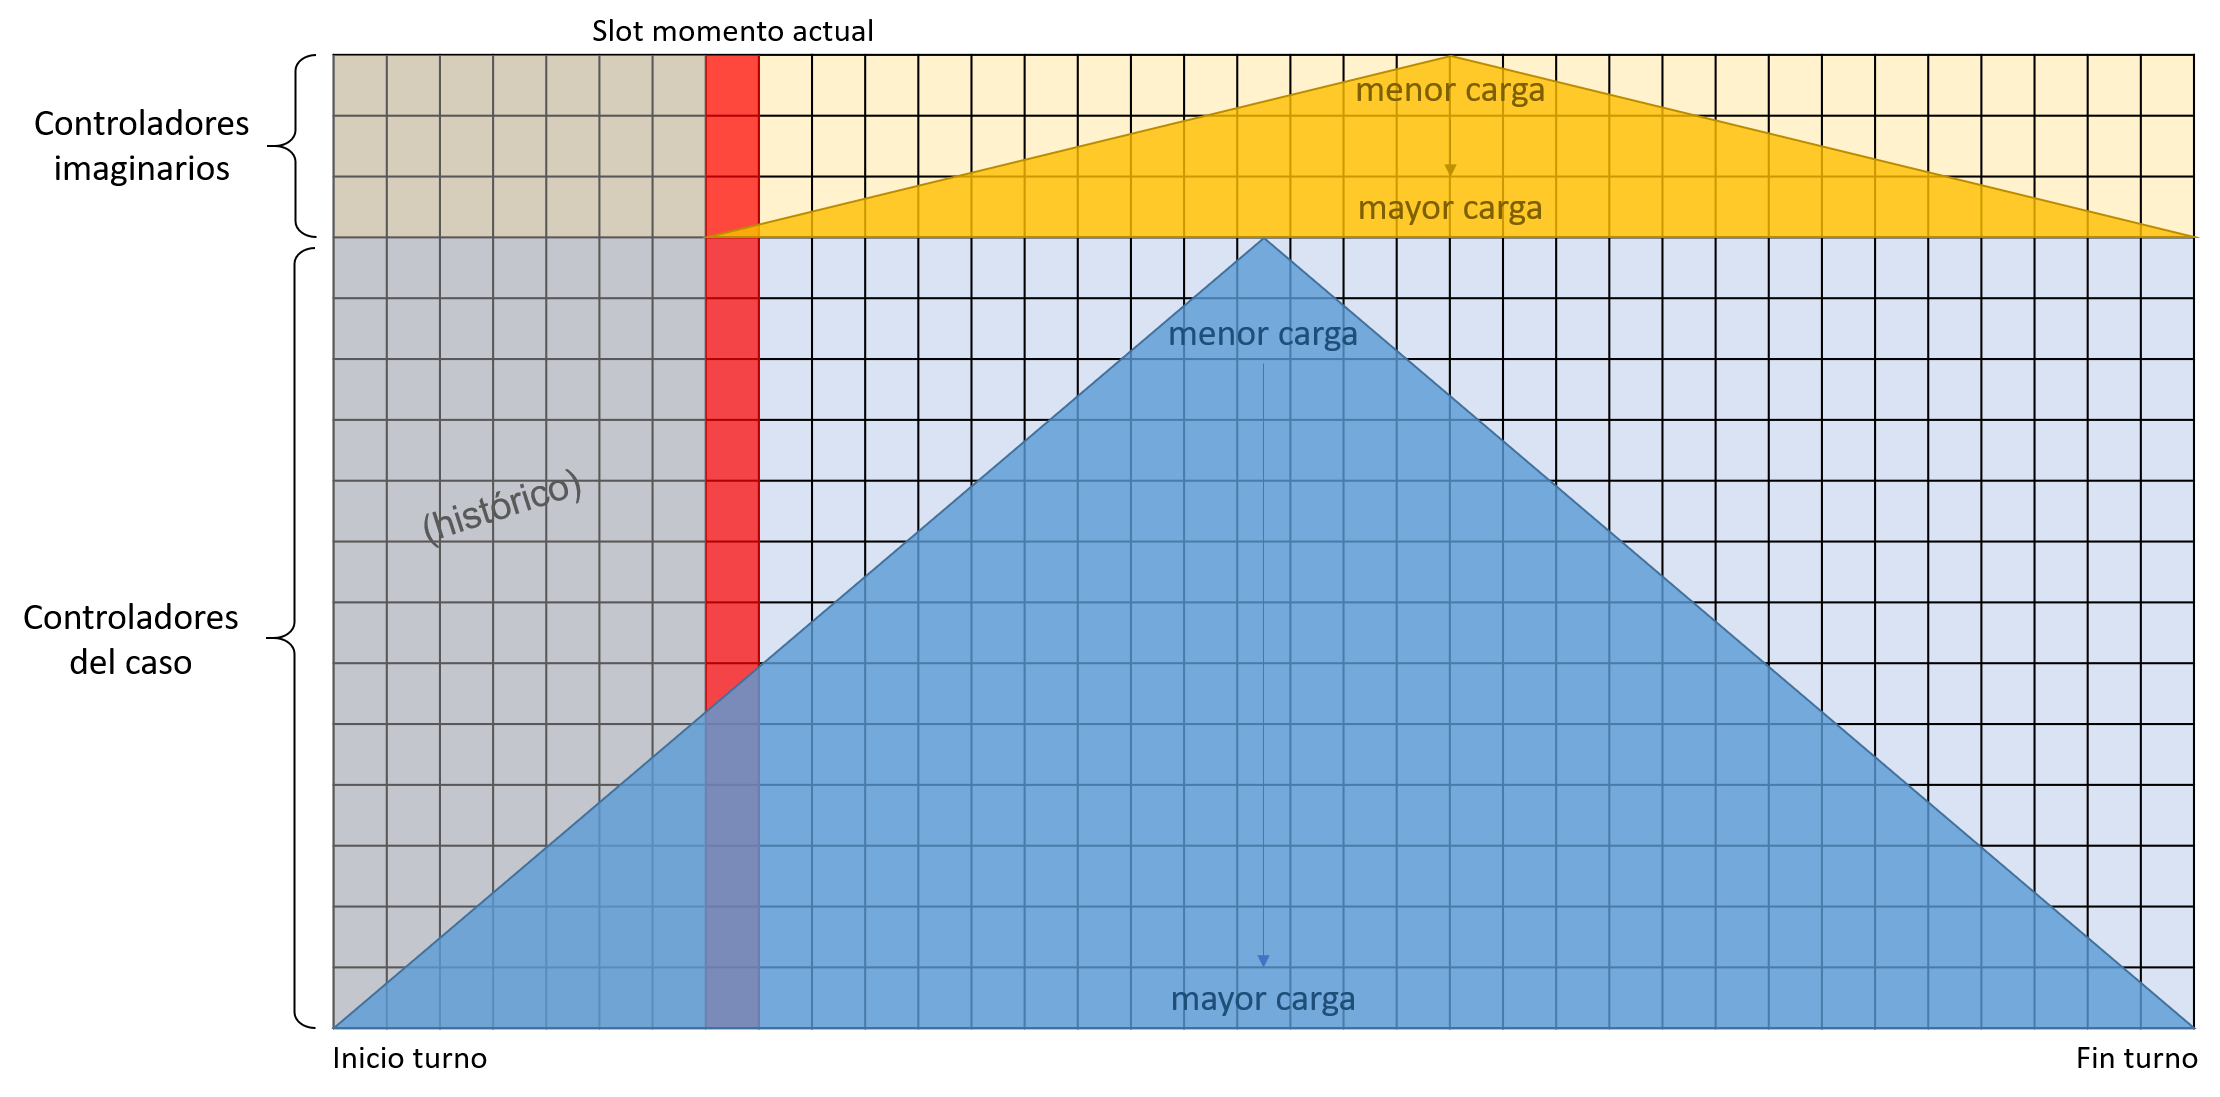
\includegraphics[width=\linewidth]{capitulos/Capitulo3-Metodologia-propuesta/recursos/estructura-piramidal}
	\caption{Esquema de la estructura piramidal de las soluciones}
	\label{fig:3:estructura-piramidal}
\end{figure}

Una vez alcanzado el valor 1 de este primer objetivo, la ordenación deja de ser necesaria y nos podemos ahorrar ese tiempo de cómputo bastante significativo, pues todo método de ordenación es bastante costoso, del orden de $O(n^2)$.

La segunda función objetivo~\ref{O2} tratará de minimizar\footnote{En realidad la expresión se transforma en términos de maximización pero la esencia es esa.} el número de restricciones del dominio incumplidas ---definidas en la \autoref{sec:4:RD}---, favoreciendo la factibilidad de la solución alcanzada. Su implementación cuenta el número de restricciones incumplidas (normalizado).

En caso de que el trabajador tenga slots fuera de turno (véase la \autoref{sec:baja-alta-controladores}) éstos serán contabilizados como descansos para que en aquellos controladores que llegan como sustitutos en momentos finales de la planificación se tenga en cuenta que no han estado trabajando y el porcentaje de descanso mínimo (Restricción \ref{RD:3:porcentaje-min-descanso}) tenga un valor coherente con la realidad.

En nuestra implementación, para ahorrar tiempo de cómputo, el conteo de las restricciones incumplidas se realiza en paralelo, aprovechando la capacidad de computación multihilo del ordenador de trabajo (véase la \autoref{sec:4:mejorando-eficiencia}).

La tercera función objetivo~\ref{O3}, implementada por vez primera para este sistema, trata de minimizar el número de cambios de sala al momento de producirse la incidencia. Esto es debido a que cuanto menos se muevan los trabajadores de su puesto, más eficiente y rápida podrá realizarse la transición desde la planificación previa (la parte inamovible de la planificación, a la izquierda del momento del cambio) y la nueva (la creada por el sistema, a partir del momento del cambio).

Para contar el número de cambios simplemente tendremos que recorrer la matriz por la columna del momento del cambio, el índice $slot_{actual}$, y compararla con la columna anterior $slot_{actual}-1$, matemáticamente lo podríamos expresar como:
%
\[
    f_3(\textbf{x}) = \frac{1}{nATC} \sum_{i=1}^{nATC}
    \begin{cases}
        1\,, & \quad \textrm{si } \textbf{x}_i^{slot_{cambio}} = \textbf{x}_i^{slot_{cambio}-1} \\
        0\,, & \quad \textrm{en otro caso }
    \end{cases}
    \,,
\]


%\[
%	f_3(x) = \frac{1}{nATC} \sum_{i=1}^{nATC} t_i
%	\; , \quad \textrm{con } t_i = \begin{cases}
%		1 & \quad \textrm{si } x_i^{slot_{actual}} = x_i^{slot_{actual}-1} \\
%		0 & \quad \textrm{en otro caso }
%	\end{cases}
%\]

con $\textbf{x}_i^j$ el sector y la posición asignados por la solución $\textbf{x}$ al controlador $i$ (fila) en el slot $j$ (columna).

Consideramos un cambio tanto cuando el sector es diferente como cuando lo es la posición, aunque sea el mismo sector.
El cociente $\sfrac{1}{nATC}$ sirve para normalizar la función y poder usarla junto con todas las demás.

La cuarta y última función objetivo~\ref{O4}, trata de lograr que las planificaciones resultantes sean parecidas a los estadillos (definidos en la \autoref{sec:3:inicializacion-soluciones}). Lo lograremos comparando para cada slot de la solución el sector asignado con aquél del slot inmediatamente a la derecha y aquel inmediatamente inferior. Matemáticamente de la siguiente forma:
%
\[
    f_4(x) = \sum_{i=1}^{nATC} \sum_{i=1}^{nSlots}
    \begin{cases}
        1\,, & \; \textrm{si } \; \textbf{x}_i^j = \textbf{x}_{i+1}^{j} \\
        \\
        1\,, & \; \textrm{si } \; \textbf{x}_i^j = \textbf{x}_{i}^{j+1}   \\
        \\
        0\,, & \; \textrm{en otro caso }
    \end{cases}
    \,,
\]

con $nSlots$ el número de slots de la instancia concreta del problema. 

Cabe destacar que, en caso de alcanzar slots
donde no sea posible comparar con posiciones inmediatamente inferior o derecha debido a que se alcance el final de la matriz, entonces ese caso (inferior o derecha) será ignorado.
%Por otra parte, para que el~\ref{O1} s
%TODO que es esto?

\paragraph{Definición de entornos} \label{paragraph:entornos}
En secciones previas se ha introducido el concepto de entorno: estructuras algorítmicas de manipulación de una solución que permiten moverse hacia otras cercanas. Por lo tanto, definen el criterio a emplear para moverse entre soluciones.

Para definir un entorno, necesitamos conocer la representación de las soluciones (recuérdese la \autoref{sec:3:representacion-soluciones}), pues en función de la misma definiremos los entornos. En nuestro caso, se trata de una representación discreta en forma matricial. Para este tipo de representaciones lo más habitual es la permutación de elementos de la solución para transformarlas en otras.

Los antecedentes respecto a las definiciones de entorno no son demasiados, Jónatan Lara Valero realizó un estudio exhaustivo desde el punto de vista matemático de los entornos del sistema \legacy{} y propuso uno nuevo con una técnica innovadora de rejilla. En su TFM, Lara describe y analiza el comportamiento de los entornos definidos por Tello et al. en~\cite{articulo1} denominados como \textit{mov3} y \textit{mov6}.

El primer movimiento, \textit{mov3}, se define algorítmicamente de la forma indicada en el \autoref{algoritmo:entorno-mov3}. Como podemos ver, consiste en probar todas las posibles combinaciones de controladores y longitudes hasta encontrar una combinación que nos permita realizar el cambio.

\begin{algorithm}[h]
    \caption{Movimiento \textit{mov3}}
    %	\algorithmicgoto~\ref{testtt}
    \label{algoritmo:entorno-mov3}

    \SetAlgoNoLine
    \SetAlgoNoEnd
    \DontPrintSemicolon
    \LinesNumbered
    %	\setstretch{1.35}
    %	\setlength{\parskip}{0.4ex}

    \KwIn{

    $s$, una solución
    %		$d$, índice de la solución inicial
    }
    \bigskip

    %	\Repeat{no queden controladores por probar}{
    %		Seleccionar un controlador $c_1$ aleatoriamente \;
    %		Elegir un periodo de trabajo de $c_1$ aleatoriamente \label{testtt} \;
    %	}

    Seleccionar un controlador $c_1$ aleatoriamente \; \label{line:c1}
    \algovspace

    Obtener lista de los periodos de trabajo continuados $L_{c_1}$
    \algovspace

    Elegir un periodo de trabajo de $L_{c_1}$ aleatoriamente \label{line:3} \;
    \algovspace

    Generar lista de amplitudes mediante múltiplos del tamaño del descanso. En nuestro sistema siempre es de 6 (véase la \autoref{capitulo:3:paso-2}), por lo que sería: $\left\lbrace 3,6,9,12\right\rbrace $ \;
    \algovspace

    Seleccionar una amplitud (granularidad) $d$ aleatoriamente de entre la lista \label{line:amplitud}\;
    \algovspace

    Seleccionar los $d$ primeros slots del periodo de trabajo $L_{c_1}$ seleccionado en el \algorefpaso{line:3}\; % paso(\ref{line:3})
    \algovspace

    Elegir aleatoriamente otro controlador $c_2$ \label{line:c2}\;
    \algovspace

    \leIf{se puede realizar el cambio de carga $L_{c_1}$ de $c_1$ a $c_2$}
    {hacer el cambio y \textbf{fin}, }
    {se elige otro $c_2$ aleatoriamente (sin repeticiones), volviendo al \algorefpaso{line:c2}}
    \algovspace

    \lIf{ningún $c_2$ admite la carga de $c_1$}{elegir otra amplitud $d$, volviendo así al \algorefpaso{line:amplitud}} %paso (\autoref{line:amplitud})}
    \algovspace

    \lIf{ninguna amplitud permite un cambio válido}{elegir otro controlador $c_1$, volviendo al \algorefpaso{line:c1}} % paso (\ref{line:c1})}
    \algovspace

    \lIf{aun así no es posible en ninguna combinación}{\Return $\emptyset$}
    \algovspace
\end{algorithm}


El movimiento \textit{mov6} consiste simplemente en la repetición del anterior dos veces para potenciar la capacidad exploratoria del sistema.

Lara en su TFM propone además los movimientos en una o varias rejillas, que tratan de mantener la estructura vertical que tienen las soluciones debido a los patrones regulares que presentan los estadillos empleados para definir la solución inicial:

\begin{quotation} {\itshape
%	Los movimientos en rejilla parten de una idea básica: mantener la estructura
%	vertical de las soluciones iniciales. [...] La construcción de las soluciones iniciales a partir de plantillas hace que tengan ciertas regularidades La estructura vertical es esta regularidad. +
%	Los cambios en las asignaciones se hacen con regularidad y solo la sectorización puede romper esta regularidad.

<<Los movimientos \textit{mov3} y \textit{mov6} rompen la estructura vertical de las soluciones
iniciales salvo que las amplitudes, la longitud de los descansos y la sectorización sean
compatibles entre sí, caso que no se da en muchas situaciones.

Para solventar este problema definimos el movimiento \textit{mov12}. En este movimiento,
se crea una rejilla a partir de la solución inicial que limita los intercambios
que pueden hacerse entre controladores. Una rejilla no será más que una serie de
puntos que dividirán el turno en intervalos, no necesariamente iguales en tamaño. El
movimiento \textit{mov12} consistirá siempre en intercambiar uno de estos intervalos entre
dos controladores.>>}

    \hfill ---Jónatan Lara Valero~\cite{tesis-jonatan}
\end{quotation}

A su vez propone otros movimientos como variaciones de este, pero para este TFM únicamente hemos considerado su propuesta del uso de rejillas simple como un tipo de entornos que hemos definido. Este tipo de entornos limitan los intercambios de carga de trabajo permitidos a unas franjas de intervalos concretas. Véase la \autoref{fig:representacion-rejilla} para comprender visualmente cómo se constituye una rejilla a partir de una solución.

\begin{figure}
    \centering
    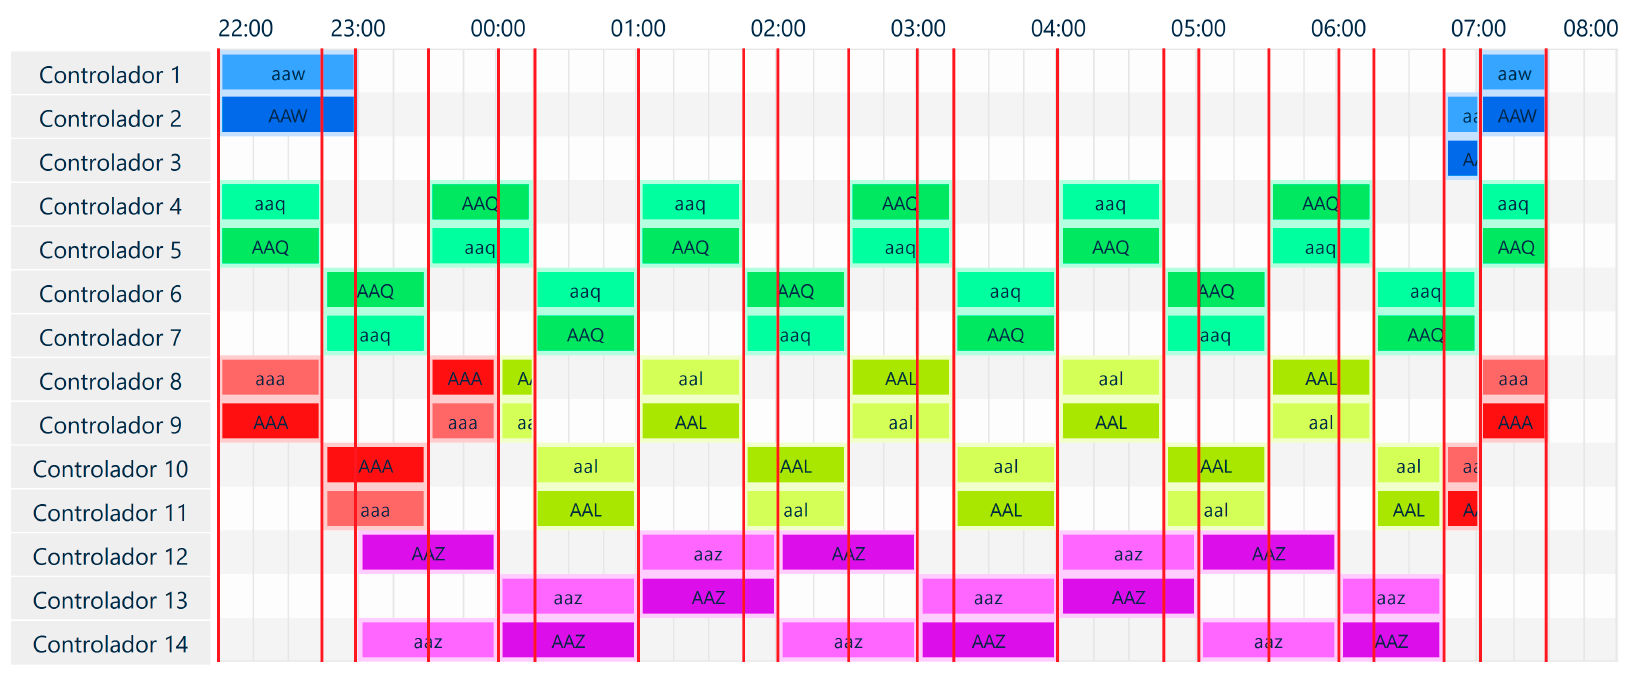
\includegraphics[width=\linewidth]{representacion-rejilla}
    \caption[Representación gráfica de una rejilla]{Representación gráfica de una rejilla. Fuente:~\cite{tesis-jonatan}}
    \label{fig:representacion-rejilla}
\end{figure}

Si bien no forma parte de este TFM, pues no se trata de trabajo propio, debido a que en el \autoref{capitulo:5} se hacen comparaciones entre las dos metaheurísticas definidas, consideramos importante en esta sección destacar que, los entornos definidos para el sistema \legacy{} fueron actualizados siguiendo la codificación definida (véase la \autoref{sec:3:representacion-soluciones})
y el SA fue ejecutado empleando todos ellos. El estudio concluyó con que el entorno que mejores resultados ofrecía para el SA es el \textit{mov15}, uno de los propuestos por Lara en~\cite{tesis-jonatan}, de tipo rejilla con la variación de que permite intercambiar más de un intervalo a la vez, entre 1 y 3 siempre y cuando estén consecutivos.
% TODO: poner o referenciar en el capítulo 5!!!

Por otro lado, para el sistema \legacy{} también se desarrolló un VNS previamente: Pablo Lozano Santiuste propuso unas estructuras de entornos que intercambiaban carga a nivel de slot, repitiéndose sucesivas veces hasta que no fuese posible realizar el cambio. De esta forma, se intercambiaría toda la carga posible de los dos controladores seleccionados aleatoriamente. 

Lozano en su TFM~\cite{tesis-pablo} emplea 4 tipos de entornos cuyas diferencias residen en las restricciones de entorno de cada una: para poder realizar el cambio o bien es necesario que el primero trabaje y en segundo descanse o bien que ambos trabajen; y otros dos equivalentes pero con la restricción adicional de que el trabajo del segundo controlador sea en el mismo sector que el primero previamente, de forma que se continúe el trabajo.

Para este TFM se han empleado ideas de todos ellos y se han definido tres tipos de entornos, cada uno con un principio diferente:

\begin{itemize}
    \item \textbf{Movimientos de máxima carga} \textit{(movMaxCarga)}: se basan en el traspaso de la mayor carga posible de trabajo entre los controladores.

    \item \textbf{Movimientos en rejilla} \textit{(movRejilla)}: permiten el traspaso de carga sin romper la estructura de la solución.

    \item \textbf{Movimiento libre} \textit{(movLibre)}: si no es posible un intercambio mediante ninguno de los anteriores, trataremos de tomar intervalos más pequeños de carga.
\end{itemize}

Como podemos ver, los dos primeros no tienen libertades de movimiento, sino que deberán mover un número de slots concreto, nunca menor que la carga continuada o la sección limitada por la rejilla. Para no limitar el espacio de soluciones, añadimos el último, que permite esa libertad en cuanto al tamaño. A continuación, describiremos cada uno de ellos.

La idea inicial consiste en emplearlos en el orden descrito, de forma que primero se quite la máxima carga del controlador superior y si no es posible, se utilicen rejillas, y finalmente sin restricciones de entorno. No obstante, empíricamente descubrimos que esto no siempre es lo más óptimo, tal y como podemos observar en la \autoref{sec:5:resultados-ajuste}.

\subparagraph{Movimientos de máxima carga}
\label{entorno:movMaxCarga}

\textbf{Objetivo:} Intentar pasar toda la carga de trabajo continuado.

\textbf{Comportamiento:} Se intenta pasar toda la máxima carga posible de trabajo de $c_1$ a $c_2$

%\textbf{Algoritmo:}
\RestyleAlgo{ruled}
\SetAlgoNoLine
\LinesNumbered
\SetAlgoNoEnd
\DontPrintSemicolon
\begin{algorithm}[h]
    \label{algoritmo:movMaxCarga}
    
   	\caption{Movimiento de máxima carga}
    	
    \SetAlgoNoEnd
    Se elige arbitrariamente un controlador $c_1$ (en caso de existir algún imaginario, en lugar de arbitrariamente, se toma en orden partiendo \newline del primer imaginario) \label{line:maxcarga:paso1}\;
    \algovspace

    Obtener los intervalos de trabajo continuo de $c_1$\;
    \algovspace

    Elegir un intervalo de trabajo aleatoriamente \label{line:maxcarga:trabajo}\;
    \algovspace

    Elegir arbitrariamente un controlador $c_2$ \label{line:maxcarga:c2}\;
    \algovspace

    \If{se cumple la restricción de dominio \ref{RD:acreditacion-valida} (que la acreditación sea válida) y las restricciones del entorno \label{line:maxcarga:restricciones}}
    {traspasar carga y \textbf{fin}}
    %	\footnote{Es decir, que ambos trabajadores estén acreditados para llevar a cabo el trabajo del otro controlador}
    \algovspace

    \textbf{en caso de\,} \underline{no cumplirse alguna restricción}, probar con otro $c_2$ volviendo al \autoref{line:maxcarga:c2}\;
    \algovspace

    \textbf{en caso de\,} \underline{haber probado todos los $c_2$}, tomar otro intervalo de trabajo y volver al \autoref{line:maxcarga:trabajo}\;
    \algovspace

    \textbf{en caso de\,} \underline{haber probado todos los intervalos de trabajo}, volver al \autoref{line:maxcarga:paso1} hasta probar todos los $c_1$\;
    \algovspace
\end{algorithm}

\textbf{Restricciones de entorno (y nombre):}
\begin{enumerate}[align=parleft, labelsep=2cm, itemindent=5em, font=\itshape]
    \item[MovMaxCarga]\mbox{}\\No hay restricciones.

    \item[MovMaxCarga\_1]\mbox{}\\
    $c_1$ debe tener trabajo en el intervalo elegido. \\
    $c_2$ debe estar descansando en el intervalo elegido.

    \item[MovMaxCarga\_2]\mbox{}\\
    $c_1$ y $c_2$ deben tener trabajo en el intervalo elegido. \\
    El sector y la posición de trabajo de $c_1$ debe ser la misma que la de $c_2$.

    \item[MovMaxCarga\_3]\mbox{}\\
    $c_1$ y $c_2$ deben tener trabajo en el intervalo elegido. \\
    El sector de $c_1$ debe ser el mismo que el de $c_2$, pero la posición del trabajo no tiene por qué.

    \item[MovMaxCarga\_4]\mbox{}\\
    $c_1$ y $c_2$ deben tener trabajo en el intervalo elegido. \\
    El sector y la posición de trabajo podrán ser diferentes.
\end{enumerate}

\subparagraph{Movimientos en rejilla}
\label{entorno:movRejilla}

\textbf{Objetivo:} Intentar pasar la carga de trabajo de forma controlada para no romper la estructura de la solución.

\textbf{Comportamiento:} El cambio de carga de trabajo se realiza únicamente entre intervalos limitados por las rejillas. La estructura de las rejillas puede cambiar en cada iteración debido a los demás movimientos, por lo que se debe ejecutar la fragmentación del controlador en las rejillas en cada ejecución del movimiento.

%\textbf{Algoritmo:}
%\RestyleAlgo{plain}
%\SetAlgoNoLine
%\LinesNumbered
%\SetAlgoNoEnd
%\DontPrintSemicolon
\begin{algorithm}[h]
	
	\caption{Movimiento en rejilla}

	\label{algoritmo:movRejilla}
    \SetAlgoNoEnd
    Se elige arbitrariamente un controlador $c_1$ (en caso de existir algún imaginario, en lugar de arbitrariamente, se toma en orden partiendo \newline del primer imaginario) \label{line:rejilla:paso1}\;
    \algovspace

    Obtener rejilla\;
    \algovspace

    Elegir un intervalo de la rejilla aleatoriamente \label{line:rejilla:trabajo}\;
    \algovspace

    Elegir arbitrariamente un controlador $c_2$ \label{line:rejilla:c2}\;
    \algovspace

    \If{se cumple la restriccion de dominio \ref{RD:acreditacion-valida} y las restricciones del entorno \label{line:rejilla:restricciones}}{traspasar carga y \textbf{fin}}
    %	\footnote{Es decir, que ambos trabajadores estén acreditados para llevar a cabo el trabajo del otro controlador}
    \algovspace

    \textbf{en caso de\,} \underline{no cumplirse alguna restricción}, probar con otro $c_2$ volviendo al \autoref{line:rejilla:c2}\;
    \algovspace

    \textbf{en caso de\,} \underline{haber probado todos los $c_2$}, tomar otro intervalo de trabajo de la rejilla arbitrariamente, volviendo al \autoref{line:rejilla:trabajo}\;
    \algovspace

    \textbf{en caso de\,} \underline{haber probado todos los intervalos de trabajo}, volver al \autoref{line:rejilla:paso1} hasta probar todos los $c_1$\;
    \algovspace
\end{algorithm}

\textbf{Restricciones de entorno (y nombre):}
\begin{enumerate}[align=parleft, labelsep=2cm, itemindent=5em, font=\itshape]
    \item[MovRejilla]\mbox{}\\No hay restricciones.

    \item[MovRejilla\_1]\mbox{}\\
    Seleccionamos aleatoriamente uno de los intervalos de las rejillas que cumplan:
    $c_1$ debe tener trabajo en el intervalo elegido. \\
    $c_2$ debe estar descansando en el intervalo elegido.

    \item[MovRejilla\_2]\mbox{}\\
    $c_1$ y $c_2$ deben tener trabajo en el intervalo elegido. \\
    El sector y la posición de trabajo de $c_1$ deberán ser la misma que la de $c_2$.

    \item[MovRejilla\_3]\mbox{}\\
    $c_1$ y $c_2$ deben tener trabajo en el intervalo elegido. \\
    El sector de $c_1$ deberá ser el mismo que el de $c_2$, pero la posición del trabajo no tiene por qué.

    \item[MovRejilla\_4]\mbox{}\\
    $c_1$ y $c_2$ deben tener trabajo en el intervalo elegido. \\
    El sector y la posición de trabajo podrán ser diferentes.
\end{enumerate}

\subparagraph{Movimiento libre (\textit{movLibre})}
\label{entorno:movLibre}

\textbf{Objetivo:} Intentar pasar la carga de trabajo en tamaños menores, permitiendo romper la estructura.

\textbf{Comportamiento:} Prueba tamaños de mayor a menor hasta que se pueda hacer el cambio

Para el caso de \textit{movLibre} no se han definido restricciones de dominio.

%\textbf{Algoritmo:}
%\RestyleAlgo{plain}
%\SetAlgoNoLine
%\LinesNumbered
%\SetAlgoNoEnd
%\DontPrintSemicolon
\begin{algorithm}[h]
    \label{algoritmo:movLibre}
    
   	\caption{Movimiento libre}
    	
    \SetAlgoNoEnd
    Elegir aleatoriamente un controlador $c_1$  \label{line:libre:paso1}\;
    \algovspace

    Obtener intervalos de trabajo continuados de $c_1$\;
    \algovspace

    Elegir un intervalo de trabajo aleatoriamente \label{line:libre:trabajo}\;
    \algovspace

    Seleccionar un subintervalo desde el inicio del intervalo hasta un cierto tamaño que será inicialmente el máximo y se irá reduciendo en 1 slot \newline cada vez que no encuentre opción de hacer el traspaso de carga \label{line:libre:subintervalo}\;
    \algovspace

    Elegir arbitrariamente un controlador $c_2$ \label{line:libre:c2}\;
    \algovspace

    \If{se cumple la restriccion de dominio \ref{RD:acreditacion-valida}}{traspasar carga y \textbf{fin}}
    %	\footnote{Es decir, que ambos trabajadores estén acreditados para llevar a cabo el trabajo del otro controlador}
    \algovspace

    \textbf{en caso de\,} \underline{no cumplirse alguna restricción}, probar con otro $c_2$ volviendo al \autoref{line:libre:c2}\;
    \algovspace

    \textbf{en caso de\,} \underline{haber probado todos los $c_2$}, reducir el tamaño del subintervalo y volver al \autoref{line:libre:subintervalo}\;
    \algovspace

    \textbf{en caso de\,} \underline{haber reducido al mínimo (1 slot) el tamaño del subintervalo}, se elige arbitrariamente otro periodo de trabajo continuado, volviendo así al \autoref{line:libre:trabajo}\;
    \algovspace

    \textbf{en caso de\,} \underline{haber probado todos los intervalos de trabajo}, volver al \autoref{line:libre:paso1} hasta probar todos los $c_1$\;
    \algovspace
\end{algorithm}


\paragraph{Búsqueda diversificada/intensificada} \label{capitulo:3:busqueda-divers-intens}
Ya hemos visto que la búsqueda va orientada hacia unos objetivos, y es el valor del fitness quien permite evaluar y cuantificar cuánto se acercan a ellos. Por otro lado, para poder moverse entre soluciones, de forma que podamos aumentar
el valor del fitness, se emplean varios entornos, definidos \hyperref[paragraph:entornos]{en la sección anterior}.

En la definición de una metaheurística dos características juegan un papel importante: la intensificación (o explotación) y la diversificación (o exploración). En la \textit{intensificación}, trataremos de explorar regiones prometedoras del espacio de soluciones, dando uso a la información prometedora de la solución para obtener mejores soluciones, mientras que en la \textit{diversificación} trataremos de explorar regiones del espacio más amplias, para asegurarse de que la búsqueda no quede atrapada en un óptimo local de una región concreta del espacio.

Ambas técnicas enfocan el problema de la mejora de la solución actual de dos formas opuestas. Una buena metaheurística
hace uso de ambas de forma equilibrada, si bien las basadas en una solución suelen ser más explotativas y las poblacionales más exploratorias.

\begin{figure}
    \centering    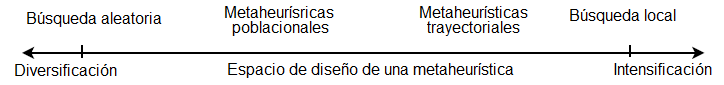
\includegraphics[width=\linewidth]{intensifiaction-vs-diversification}
    \caption[Intensificación vs diversificación]{Intensificación vs diversificación. Fuente:~\cite{sota:metaheuristicas-design-impl}}
    \label{fig:intensifiaction-vs-diversification}
\end{figure}

La metaheurística VNS es considerablemente explotativa, pero permite dar juego a estas componentes de tres posibles maneras:
\begin{enumerate}[label=\alph*.]
    \item Tipo de VNS: VND, BVNS, RVNS\ldots
    \item Orden de los entornos: hacia adelante, hacia atrás, etc.
    \item Naturaleza de selección de los entornos: determinista, probabilístico
\end{enumerate}

Vamos a analizarlos por separado en los siguientes párrafos.

El \textbf{tipo de VNS} es la forma más clara y sencilla de ajustar la capacidad exploratoria/explotatoria de la búsqueda. Si partimos de la definición básica del VNS, el \textit{Basic VNS} (recuérdese mediante el \autoref{algoritmo:Basic-VNS} a principio del capítulo) podemos ver claramente que la componente de búsqueda local es puramente intensificación, mientras que la componente de \textit{shaking} es únicamente exploración mediante una perturbación aleatoria. Esta última es precisamente la técnica más usual para introducir exploración en una metaheurística. La \autoref{fig:esquema-idea-basica-perturbacion} ilustra cómo permite salir de la zona ya explotada a otras potencialmente mejores.

Si eliminamos la componente de búsqueda local, el \textit{Reduced VNS}, potencia la exploración, mientras que si eliminamos la componente estocástica, el \textit{VND}, se potencia la capacidad de explotación.
En el caso del \textit{General VNS}, potenciamos la capacidad de exploración, pues si bien un VND es meramente determinista, a diferencia de una búsqueda local simple, emplea más de un entorno y cada uno de ellos llega a diferentes puntos del espacio de búsqueda.

Por último, el SVNS tiene por fundamento elegir soluciones peores para mejorar su eficiencia explorando por otros lugares menos prometedores, por lo que claramente potencia una capacidad exploratoria extra en la búsqueda.

\begin{figure}
    \centering    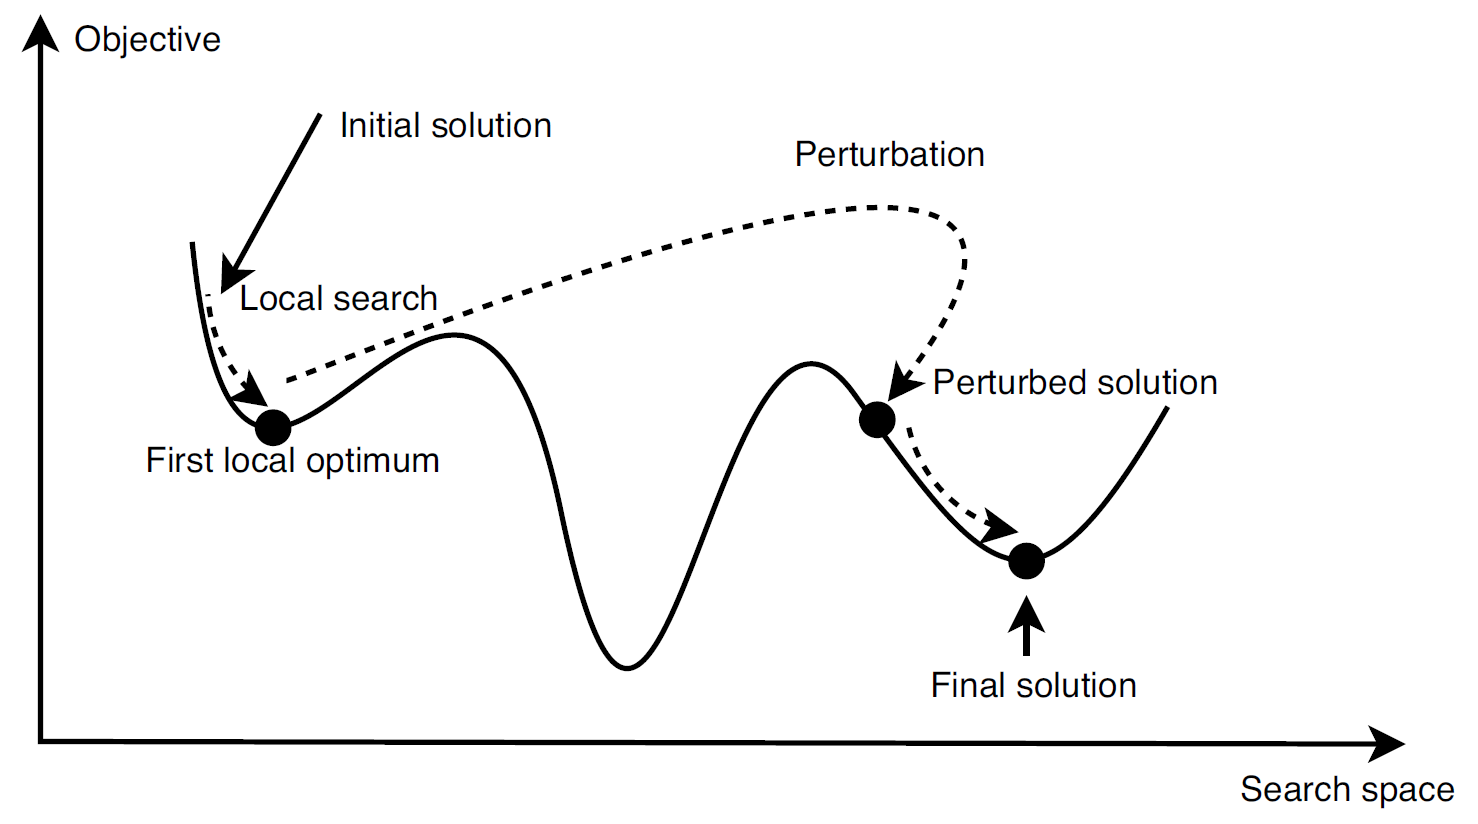
\includegraphics[width=.8\linewidth]{esquema-idea-basica-perturbacion}
    \caption[Representación gráfica de la idea de una perturbación aleatoria en un proceso de búsqueda genérico]{Representación gráfica de la idea de una perturbación aleatoria en un proceso de búsqueda de minimización genérico. Fuente:~\cite{sota:metaheuristicas-design-impl}}
    \label{fig:esquema-idea-basica-perturbacion}
\end{figure}

En segundo lugar, el \textbf{orden de los entornos} puede ser muy relevante a la hora de explorar y explotar el espacio de búsqueda, puesto que si en primer lugar la búsqueda opta por entornos más intensificadores, entonces esta dará preferencia a explotar la solución hasta que no sea posible mejorarla aún más, en cuyo caso, empleará el resto de entornos menos intensificadores y más exploratorios. Por ello tendremos que clasificar los entornos definidos anteriormente (véase la \autoref{paragraph:entornos}) en función de la característica que potencian más.
%La lista de entornos se puede recorrer de varias formas, hacia adelante ($1,\dots,k_{max}$), hacia adelante ($k_{max},\dots,1$) o con un salto, pero sin más

Se ha considerado los entornos \hyperref[entorno:movMaxCarga]{\textit{movMaxCarga}} y \hyperref[entorno:movLibre]{\textit{movLibre}} como más exploratorios, pues permiten moverse hacia soluciones más lejanas en el primero, y más difíciles de alcanzar por los demás en el caso del segundo. Por otro lado, el entorno \hyperref[entorno:movRejilla]{\textit{movRejilla}} se considera más intensificador, pues está condicionado a cambios muy concretos y limitados de la solución.

Esta clasificación es importante para la tercera y última técnica para ajustar la diversificación/intensificación del sistema: la \textbf{naturaleza de la selección de los entornos}. En esta tesis se han probado dos enfoques, el clásico determinista, y uno probabilístico.

El enfoque determinista recorre la lista de entornos definida para el sistema de forma convencional, en el orden definido, mientras que el enfoque probabilístico permite equilibrar el uso de entornos de cada uno de los dos tipos seleccionando uno aleatoriamente. La \autoref{fig:diagrama-flujo-naturaleza-entornos} representa  estos procesos en formato de diagrama de flujo. Como se puede apreciar, en el caso de la selección de los entornos de forma determinista únicamente se toma el entorno en orden, mientras que el probabilístico precisa de varios procesos.

\begin{figure}
    \centering    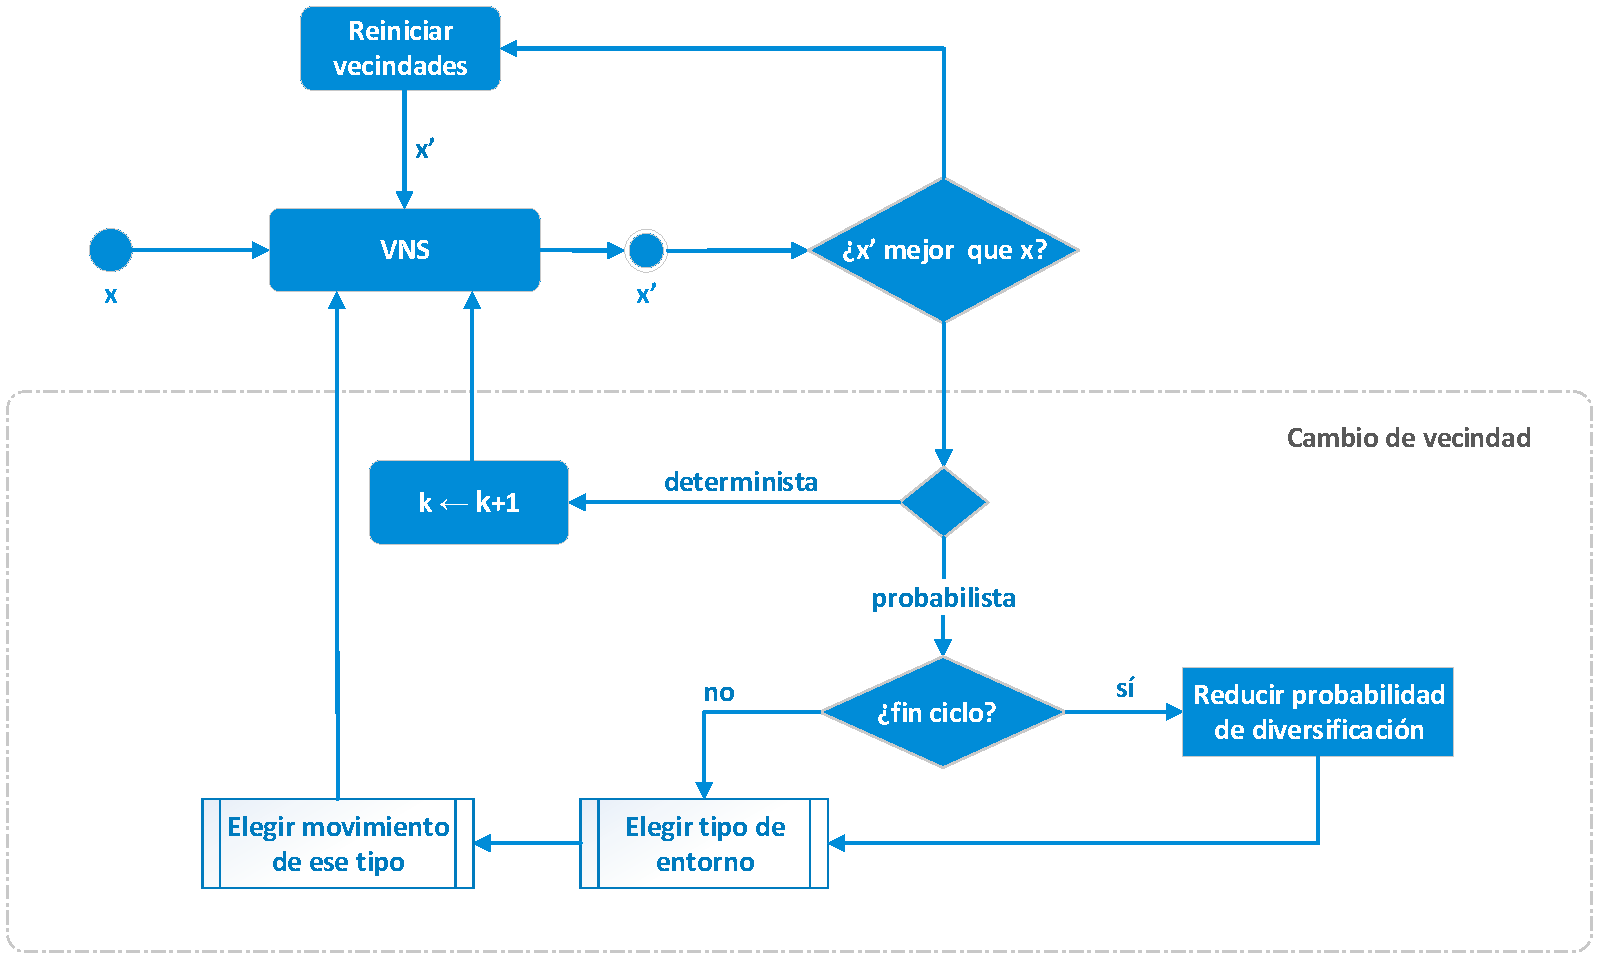
\includegraphics[width=\linewidth]{diagrama-flujo-naturaleza-entornos-bold}
    \caption{Diagrama de flujo del proceso de selección de la naturaleza de entornos}
    \label{fig:diagrama-flujo-naturaleza-entornos}
\end{figure}

En primer lugar, tenemos una probabilidad de diversificación (la probabilidad de intensificación es la complementaria, $1-p$), que irá variando cada cierto número de iteraciones que hemos denominado ciclos.

Con esa probabilidad elegimos uno de los tipos de entornos: diversificadores o intensificadores. Como es probabilístico se usará cualquiera de ambos, pero con mayor probabilidad uno que otro. Una vez escogido el movimiento (entorno), este no podrá volver a ser elegido hasta que todos los entornos pertenecientes a su grupo hayan sido utilizados (de esta forma evitamos repeticiones y garantizamos que todos sean utilizados).

La idea es tratar de que al principio las soluciones analizadas sean más diversas entre sí y a medida que la ejecución avanza se vaya reduciendo la diversificación, dando paso a la intensificación de la mejor solución alcanzada, siempre de forma estocástica. Una vez obtenido el tipo de entorno probabilísticamente, se elige el movimiento (entorno) concreto de ese tipo. En caso de utilizar entornos con restricciones, estos se ejecutan de forma determinista: en el orden en el que se han definido. La \autoref{fig:esquema-entornos-probabilisticos} resume esta información gráficamente. Más detalles desde el punto de vista de implementación están disponibles en la \autoref{sec:4:detalles-sistema}.

\begin{figure}
    \centering    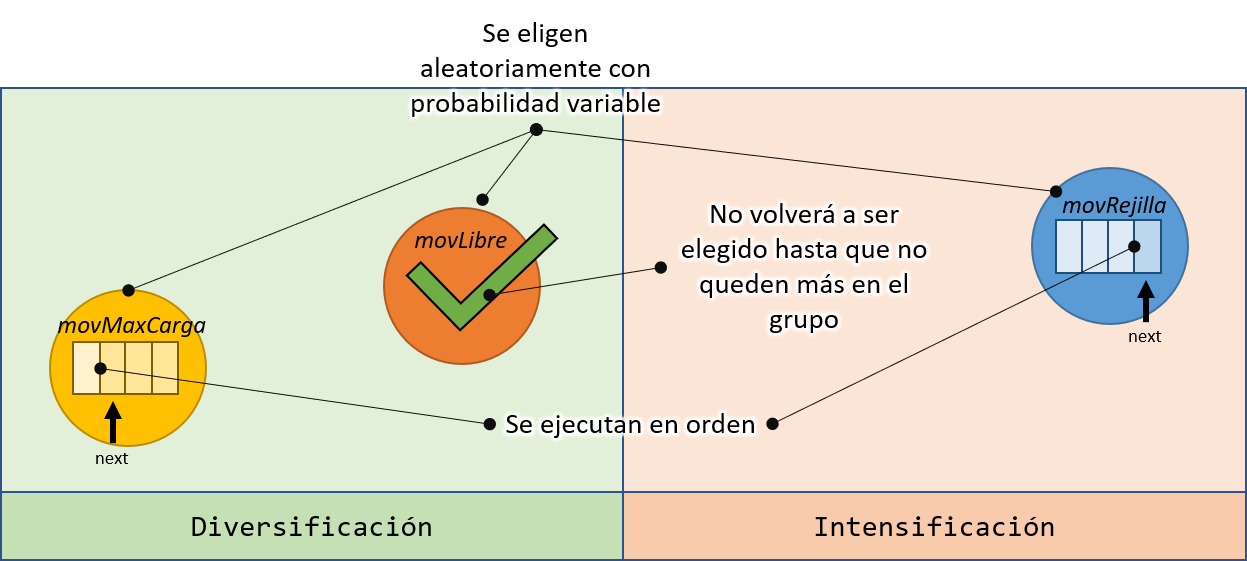
\includegraphics[width=\linewidth]{esquema-entornos-probabilisticos}
    \caption{Representación gráfica de los tipos de entornos}
    \label{fig:esquema-entornos-probabilisticos}
\end{figure}


\paragraph{Condiciones de Parada}
\label{apartado:condiciones-parada}

Sin una condición de parada, el algoritmo se estaría ejecutando de forma indefinida, por lo que siempre precisamos de al menos una.

La más intuitiva consiste en finalizar la ejecución una vez transcurrido un cierto periodo de tiempo, de esta forma si el usuario/a necesita la planificación en un plazo máximo de 10 minutos, el sistema estará buscando constantemente mejorar la solución hasta que pasen 10 minutos. Entonces, simplemente retornará al usuario/a la mejor solución alcanzada hasta el momento.

Si el sistema no requiriese de un tiempo concreto, otra posible opción sería la de detener la ejecución cuando la búsqueda no logra encontrar soluciones mejores tras el transcurso de un determinado número de iteraciones. No obstante esto tiene un problema, y es que cambios muy pequeños que manualmente no consideramos significativos el algoritmo sí los tomaría como mejoras, y un nuevo ciclo de iteraciones comenzaría, alargando tal vez innecesariamente el tiempo de ejecución. 

Por ello, la opción más común es utilizar un porcentaje mínimo de mejora (véase la \autoref{fig:porcentaje-mejora}) cuyo cálculo consiste en el incremento de la función fitness $\Delta f = |f_{inicio\, ciclo}-f_{fin\, ciclo}|$ multiplicado por 100. De esta forma, utilizamos un porcentaje mínimo que se comprueba cada cierto número de iteraciones (ciclos) que permite indicar al sistema qué mejora es significativa y cual no, finalizando la ejecución en caso de no serlo.

\begin{figure}
    \centering
    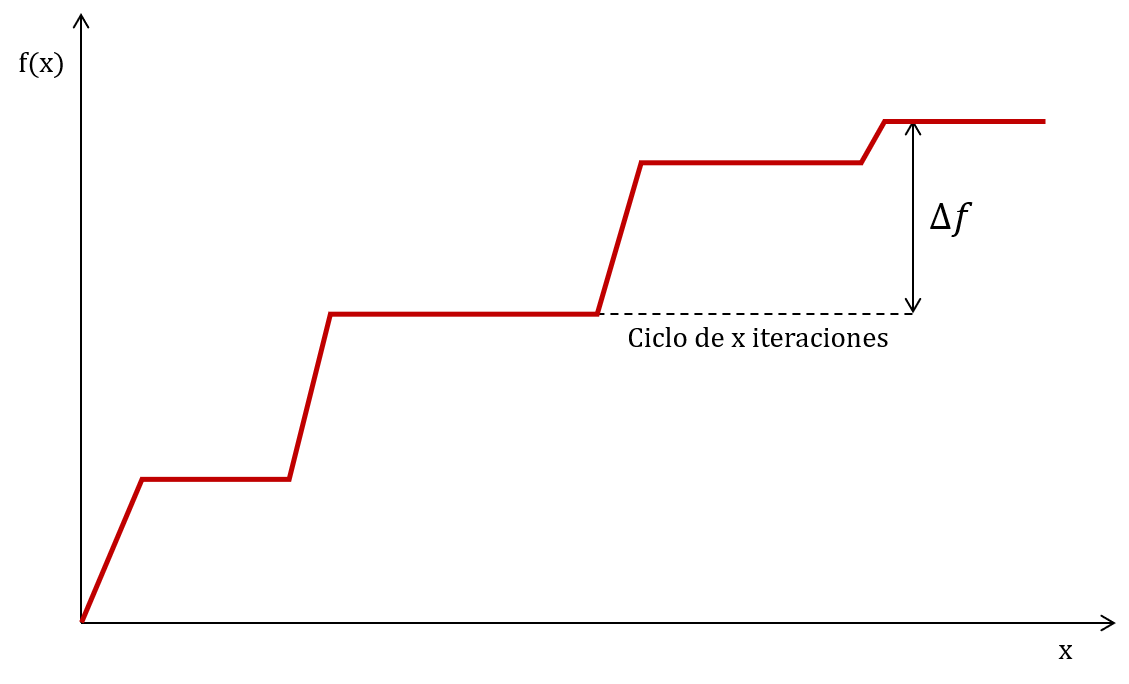
\includegraphics[width=.8\linewidth]{porcentaje-mejora}
    \caption{El porcentaje de mejora actual se calcula mediante el incremento del fitness logrado en el ciclo}
    \label{fig:porcentaje-mejora}
\end{figure}

En este sistema se han considerado ambas condiciones de parada, de forma que se detenga la ejecución tanto si no hay mejora suficiente antes de llegar al tiempo máximo como en el caso opuesto, que si bien esté mejorando ya se haya alcanzado el límite de tiempo. Ambas condiciones se evalúan tras cada cambio de vecindad como se ha representado en la \autoref{fig:esquema-fase2}.

Por otro lado, las iteraciones de la búsqueda local, tal y como se describió al comienzo de la sección, se utiliza una mixtura entre el \textit{Best Improvement} y el \textit{First Improvement}: si bien no emplea la mejor solución, tampoco emplea la primera mejor, sino que continúa la búsqueda local con la condición de parada interna definida mediante un porcentaje de tolerancia equivalente al descrito previamente.

\paragraph{Función de distancia en el Skewed-VNS}
El Skewed VNS precisa de dos parámetros adicionales: la función de distancia $d(x,x')$ y el llamado $\alpha$, ambos explicados en la \autoref{sec:vns}. El parámetro $\alpha$ se ajusta experimentalmente, y la función de distancia se ha de definir previamente.

\begin{minipage}{\textwidth}
Hemos planteado dos opciones. La distancia basada en la diferencia de sus respectivos fitness: $d_1(x,x')=f(x)-f(x')$ y basada en el número de slots diferentes entre sí:

\[
d_2(x,x')=\sum_{i=1}^{nATC} \sum_{j=1}^{nSlots}
\begin{cases}
    1\,, & \quad \textrm{si } x_i^j = {x'}_i^j \\
    0\,, & \quad \textrm{en otro caso }
\end{cases}
\]

\end{minipage}

con la peculiaridad de que en caso de que la solución no esté ordenada, se deberán de tomar los mismos controladores en cada comparación, es decir, que el lugar de comparar mediante índice se compara mediante identificador.

Para normalizar esta función (la primera ya está entre 0 y 1) se ha medido empíricamente el valor máximo posible de la función
y se ha utilizado la siguiente fórmula:
\[
    X' = \frac{X-X_{min}}{X_{max}-X_{min}} \,.
\]

Sabemos que $X_{min}=0$ y tras ejecutar la función $5\,000$ veces en total entre todos los casos disponibles, se ha obtenido un valor máximo de 400, por lo que al resultado de $d_2(x,x')$ se ha de dividir por 400 para su normalización.